\documentclass[conference]{IEEEtran}

% cd /home/samudra/Desktop/sjv_stability_feb_2022/manuscript; pdflatex main; bibtex main; pdflatex main; pdflatex main

\usepackage{cite, caption}
\usepackage{amsmath,amssymb,amsfonts, braket}
\usepackage{mathtools, braket, lipsum, bibentry}
\usepackage{graphicx}
\usepackage{textcomp}
\usepackage[usenames,dvipsnames]{xcolor}
\usepackage[utf8]{inputenc} % allow utf-8 input
\usepackage[T1]{fontenc}    % use 8-bit T1 fonts
\usepackage{booktabs}       % professional-quality tables
\usepackage{nicefrac}       % compact symbols for 1/2, etc.
\usepackage{microtype}      % microtypography
\usepackage{float}
\usepackage{enumitem}
\usepackage[caption=false,font=footnotesize]{subfig}

\def\BibTeX{{\rm B\kern-.05em{\sc i\kern-.025em b}\kern-.08em
    T\kern-.1667em\lower.7ex\hbox{E}\kern-.125emX}}
\pagestyle{plain}
\DeclarePairedDelimiter{\ceil}{\lceil}{\rceil}

\graphicspath{{../figures/}}
\newcommand{\tsh}[1]{{\color{RubineRed}#1}}
\newcommand{\tshc}[1]{{\color{RubineRed}[#1]}}
\newcommand{\Prob}{\textrm{Pr}} %% prob notation
\newcommand{\toronto}{ibmq\_toronto~}
\newcommand{\yorktown}{ibmq\_yorktown~}
\newcommand{\athens}{ibmq\_athens~}
\newcommand{\rochester}{ibmq\_rochester~}
\newcommand{\paris}{ibmq\_paris~}
\newcommand{\bogota}{ibmq\_bogota~}
\newcommand{\washington}{ibmq\_washington~}

\begin{document}
\title{Reliability of Noisy Quantum Devices
\thanks{\textit{\\ 
* Samudra~Dasgupta: dasguptas@ornl.gov, ORCID: 0000-0002-7831-745X \\
$\dagger$ Travis~S.~Humble: humblets@ornl.gov, ORCID: 0000-0002-9449-0498
}}}

\author{
\IEEEauthorblockN{Samudra~Dasgupta$^{1, 2, *}$ and Travis S.~Humble$^{1,2\dagger}$}
\IEEEauthorblockA{\textit{$^1$Bredesen Center, University of Tennessee, Knoxville, USA}\\
\textit{$^2$Quantum Science Center, Oak Ridge National Laboratory, Oak Ridge, Tennessee, USA}\\
}}


\maketitle

\begin{abstract}
TBD
\end{abstract}

\begin{IEEEkeywords}
TBD
\end{IEEEkeywords}

\section{Introduction}
\textcolor{blue}{\textit{(motivating reliability and differentiating from accuracy)}}\\
An unreliable quantum device used for computational purposes does not qualify as a quantum computer. Reliability quantification measures a device's consistency. A device is reliable if it produces consistent (similar) results under consistent conditions. Reliability captures the notions of preciseness and reproducibility but not accuracy. Said differently, high reliability does not imply high performance (or high accuracy). A device which is reliable does not imply that the device has achieved the desired performance in terms of the accuracy of results obtained.
\par
While reliability does not imply accuracy, reliability does place a limit on the overall accuracy of a circuit. A device  that is not reliable cannot be accurate and hence cannot be used either for error attribution or for prediction (and hence scientific reproducibility suffers). A reliable device is not necessarily accurate, but for a device to be called accurate and classified as a quantum computer, it must necessarily be reliable. We will quantify the notions of reliability and accuracy separately.

\textcolor{blue}{\textit{(what causes such inconsistency? the problem of noise in general)}}
Current NISQ devices suffer from high measurement errors.
Note that quantum computing is probabilistic by definition so when we say measurement error, we are not referring to variations in answer which stem from quantumness. For example, Grover's search, in the general case, has a non-zero prbability of error even if the quantum computer were perfect.
By error, we really mean systematic errors which arise due to incorrect implementation (which may be deliberate due to resource constraints and/or involuntary), and/ or hardware imperfections.

In terms of magnitude, SPAM error rates are typically higher than single-qubit rotation errors and 2-qubit entangling gate errors. There are five main sources of SPAM errors: (i) spontaneous decay (ii) energy loss to the environment (iii) inter-qubit cross-talk (iv) leakage from computational sub-space and (v) undesired coupline to external environment.

\textcolor{blue}{\textit{(defining reliability)}}\\
We will call a metric characterizing a quantum device reliable if the 95\% confidence interval for its temporal and/ or lattice variability $[a,b]$ lies within a user-defined tolerance range $[\gamma_{min}, \gamma_{max}]$ i.e.
\begin{equation}
a \leq \gamma_{\textrm{max}} \textrm{ and } b \geq \gamma_{\textrm{min}}
\end{equation}
We discuss in this study two types of reliability:
\begin{itemize}
\item temporal reliability (or across-time reliability): 95\% confidence interval for the variability across time lies within the tolerance specification. This is illustrated in Fig. (1a) and (1b).
\item lattice reliability (or inter-qubit reliability at a point-in-time): 95\% confidence interval for the variability across the lattice (or chip) at a point-in-time lies within the tolerance specification. This is illustrated in Fig. (2a) and (2b).
\end{itemize}

\textcolor{blue}{\textit{(concrete example motivating the importance of studying reliability of these metrics)}}
\begin{itemize}
\item Quality of Readout Mitigation\\
In its most basic form, readout error mitigation consists of multiplying the observed histogram count with the readout error matrix. This matrix captures the characterization of the readout noise channel. In the event the state preparation and measurement (SPAM) fidelity estimates are unreliable, then the error mitigation will become unreliable. In some cases, we may even end up making the answer even less accurate than what it was if we did not ettempt to mitigate. One way to deal with this is to characterize the channel dynamically, close to running the circuit. However, this may not be practical for large circuits. As an example, consider mitigating the readout error for a single-qubit:
\begin{equation}
\begin{pmatrix}
p_0\\p_1
\end{pmatrix}
=
\begin{bmatrix}
f_0 & 1-f_1\\
1-f_0 & f_1
\end{bmatrix}^{-1}
\begin{pmatrix}
p_0^\prime & p_1^\prime
\end{pmatrix}
\end{equation}
where 
$p_0^\prime (p_1^\prime)$ is the experimentally observed empirical probability of observing the $\ket{0} (\ket{1})$ state,
and $f_0 (f_1)$ is the SPAM fidelity ( = 1- error rate) for the $\ket{0}$ state.
If the readout channel suffers from a drift characterized by:
\begin{equation}
\begin{split}
\frac{\delta f_0}{f_0} \sim \textrm{Normal}(\mu_0 \delta t, \epsilon_0)\\
\frac{\delta f_1}{f_1} \sim \textrm{Normal}(\mu_1 \delta t, \epsilon_1)\\
\end{split}
\end{equation}
where $\epsilon_0$ and $\epsilon_1$ are zero-mean processes, then it follows that:
\begin{equation}
E(\delta p_0) = (f_0 \mu_0 p_0 - f_1 \mu_1 p_1)\delta t
\end{equation}
which captures how the readout mitigation performance deteriorates with time. This drift can be avoided by either re-calibrating the channel frequently, or asking the programmer to perform dynamic channel characterization. In both cases, $\delta t$ becomes small enough that the effect of drift can be ignored.

\item Re-calibration time-scale and margin of safety for error correction\\
According to the threshold theorem for quantum computation, a quantum circuit containing $M$ gates may be simulated with a probability of error at most $\epsilon$ using $N$ gates where:
\begin{equation}
N = M \left[\frac{\log \left(\frac{M}{c\epsilon}\right)}
{\log \left(\frac{1}{pc}\right)}
\right]^{\log d}
\end{equation}
provided $p<p_{th}$. Here, $d$ is a constant representing the maximum number of operations used in a fault-tlerant procedure to do an encoded gate and error-correction, $c=1/p_{th}$ is a constant (the pseudo-threshold probability which may need to determined experimentally or usin simulations). Now, suppose $p$ is the gate error that suffers a drift given by $p = p_0 + \mu \Delta t$. 
This gives a time-scale estimate of $\frac{1/c-p_0}{\mu}$ after which re-calibration is required so that the resource estimation does not become invalid. 
Moreover, the margin of safety for the number of gates will be given by:
\begin{equation}
\frac{\Delta N}{N} = -
\frac{\mu\log d}{[\log p_0 + \log c]}\Delta t
\end{equation}
\end{itemize}

\section{Initialization fidelity}
\subsection{Problem statement}
\textcolor{blue}{\textit{(what is our problem statement and why is it important)}}
\subsection{Method}
\subsection{Results}

\section{Gate fidelity}
\section{Addressability}
\section{Duty Cycle}

\section{Conclusion}


%%%%%%%%%%%%%%%%%%%%%%%%%
\begin{figure*} % for sub figures over two columns in 
\centering
\subfloat[Zero]{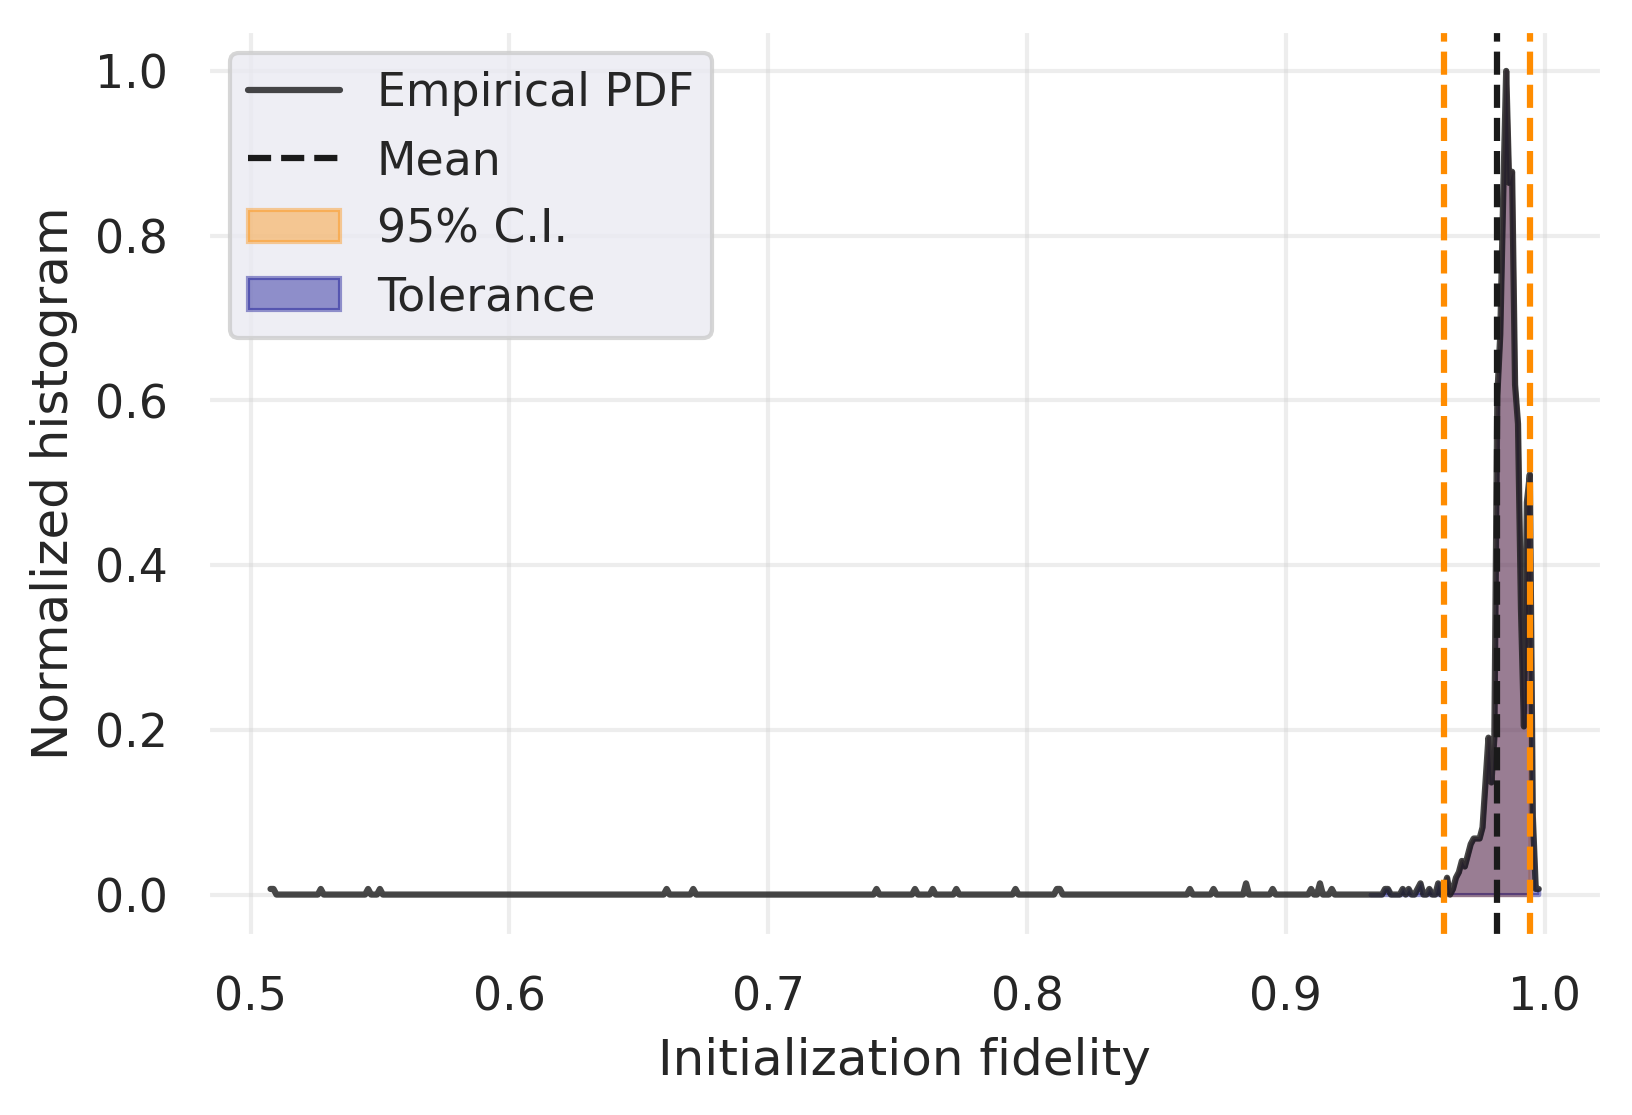
\includegraphics[width=\columnwidth]{FI_across-time.png}\label{fig:FI_across-time}}
\hfill
\subfloat[One]{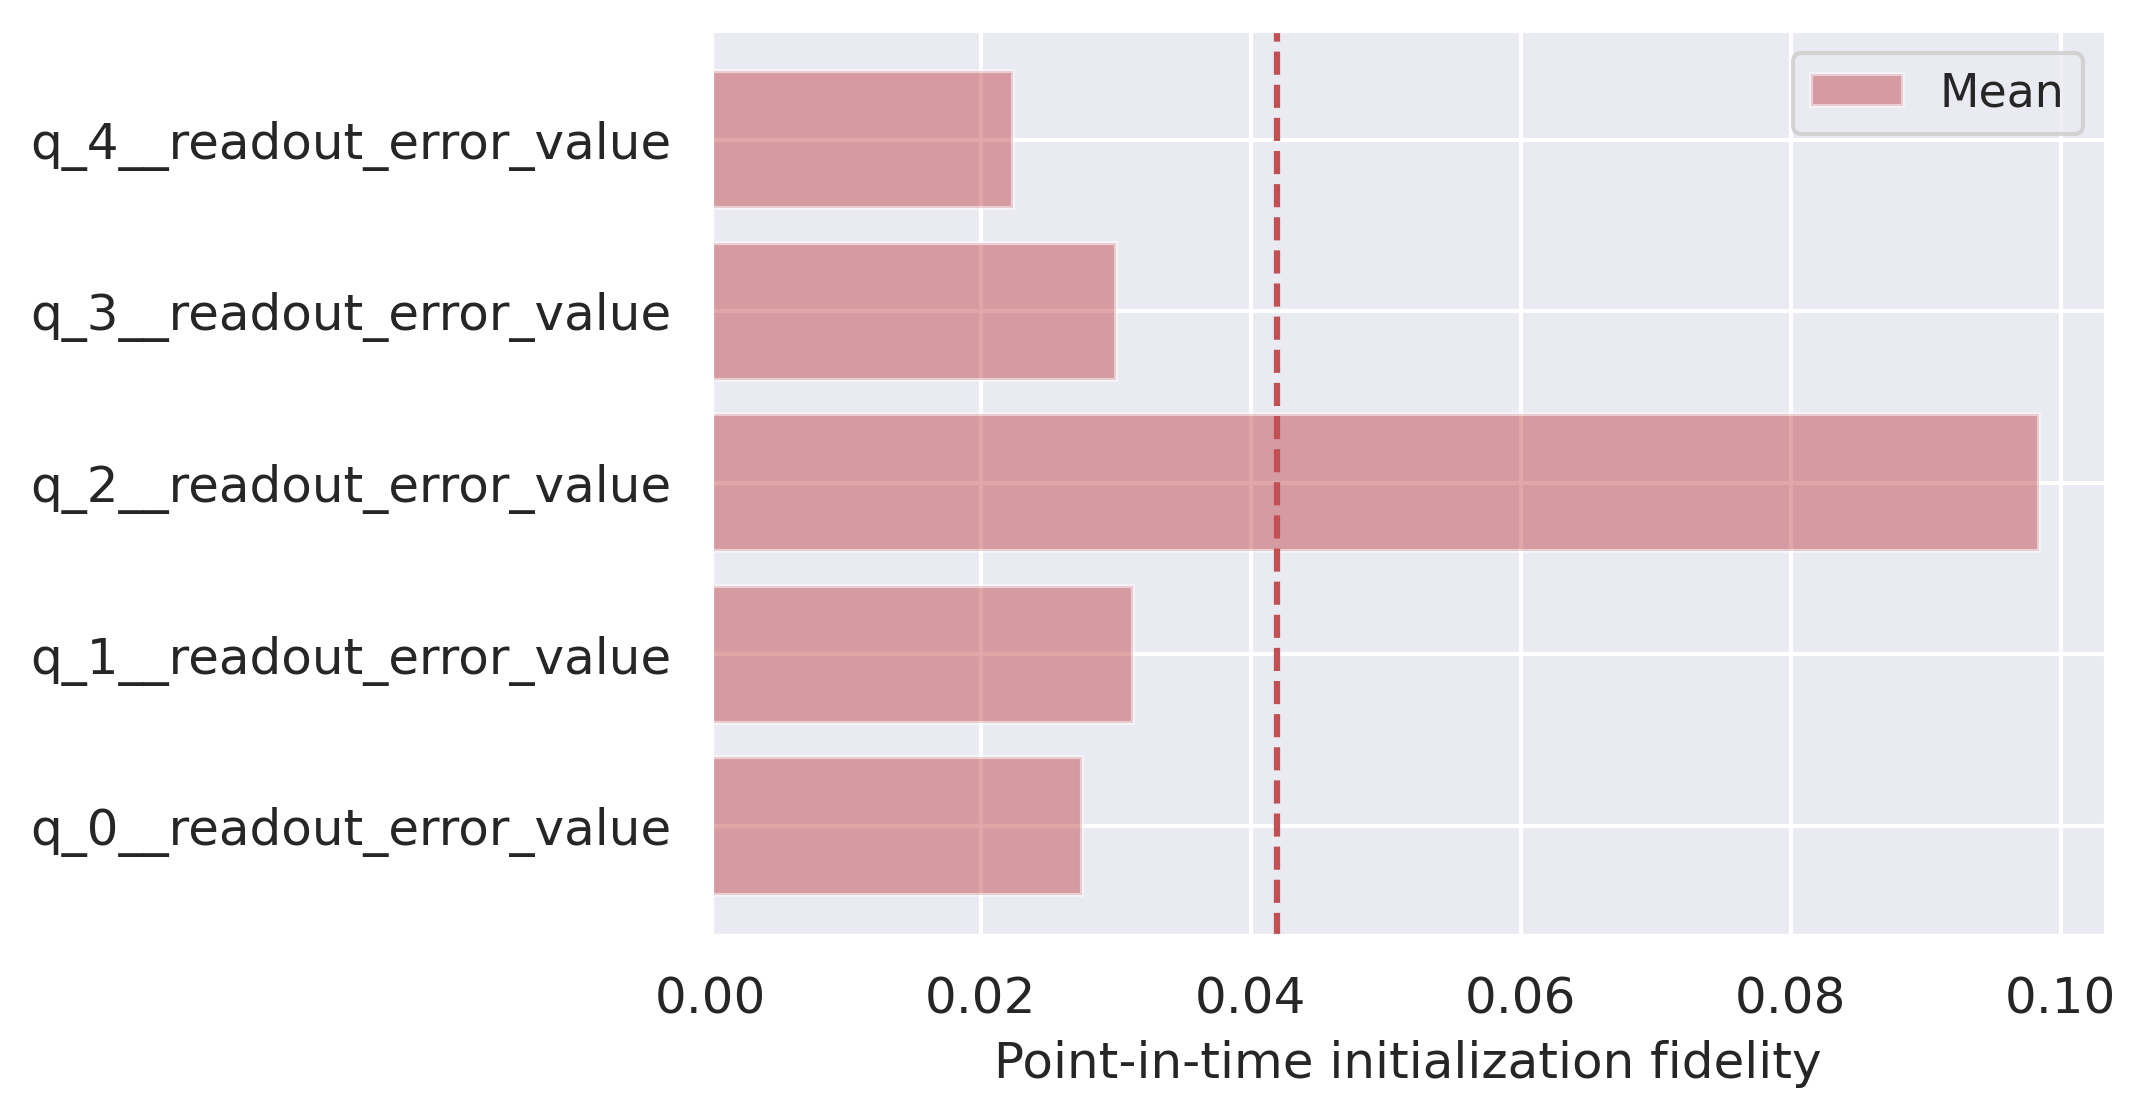
\includegraphics[width=\columnwidth]{FI_point-in-time.png}\label{fig:FI_point-in-time}}
\caption{Schematic layout}
\label{fig:tbd}
\end{figure*}
%%%%%%%%%%%%%%%%%%%%%%%%%%

\section*{Acknowledgment}
\small{
This manuscript has been authored by UT-Battelle, LLC under Contract No. DE-AC05-00OR22725 with the U.S. Department of Energy. The United States Government retains and the publisher, by accepting the article for publication, acknowledges that the United States Government retains a non-exclusive, paid-up, irrevocable, worldwide license to publish or reproduce the published form of this manuscript, or allow others to do so, for United States Government purposes. The Department of Energy will provide public access to these results of federally sponsored research in accordance with the DOE Public Access Plan. (http://energy.gov/downloads/doe-public-279access-plan).
}

\section*{IBM systems}
ONLINE:
\begin{itemize}
\item ibm\_washington
\item ibmq\_brooklyn
\item ibmq\_kolkata
\item ibmq\_montreal
\item ibmq\_mumbai
\item ibm\_cairo
\item ibm\_auckland
\item ibm\_hanoi
\item ibmq\_toronto
\item ibmq\_sydney
\item ibm\_peekskill
\item ibmq\_guadalupe
\item ibm\_perth
\item ibm\_lagos
\item ibm\_nairobi
\item ibmq\_jakarta
\item ibmq\_manila
\item ibmq\_bogota
\item ibmq\_santiago
\item ibmq\_quito
\item ibmq\_belem
\item ibmq\_lima 
\end{itemize}

RETIRED:
\begin{itemize}
\item Casablanca
\item Sydney
\item Dublin
\item Manhattan
\item Yorktown
\item Melbourne
\item Paris
\item Rome
\item Athens
\item Berlin
\item Boeblingen
\item Ourense
\item Vigo
\item Valencia
\item Almaden
\item Singapore
\item Johannesburg
\item Essex
\item Burlington
\item London
\item Rochester
\item Cambridge
\end{itemize}


%\bibliographystyle{ieeetr}
%\bibliography{stability-references-aug2-2021.bib}

\section*{Appendix}
\subsection*{Initialization Fidelity}
%%%%%%%%%%%%%%%%%%%%%%%%%
\begin{figure*} % for sub figures over two columns in 
\centering
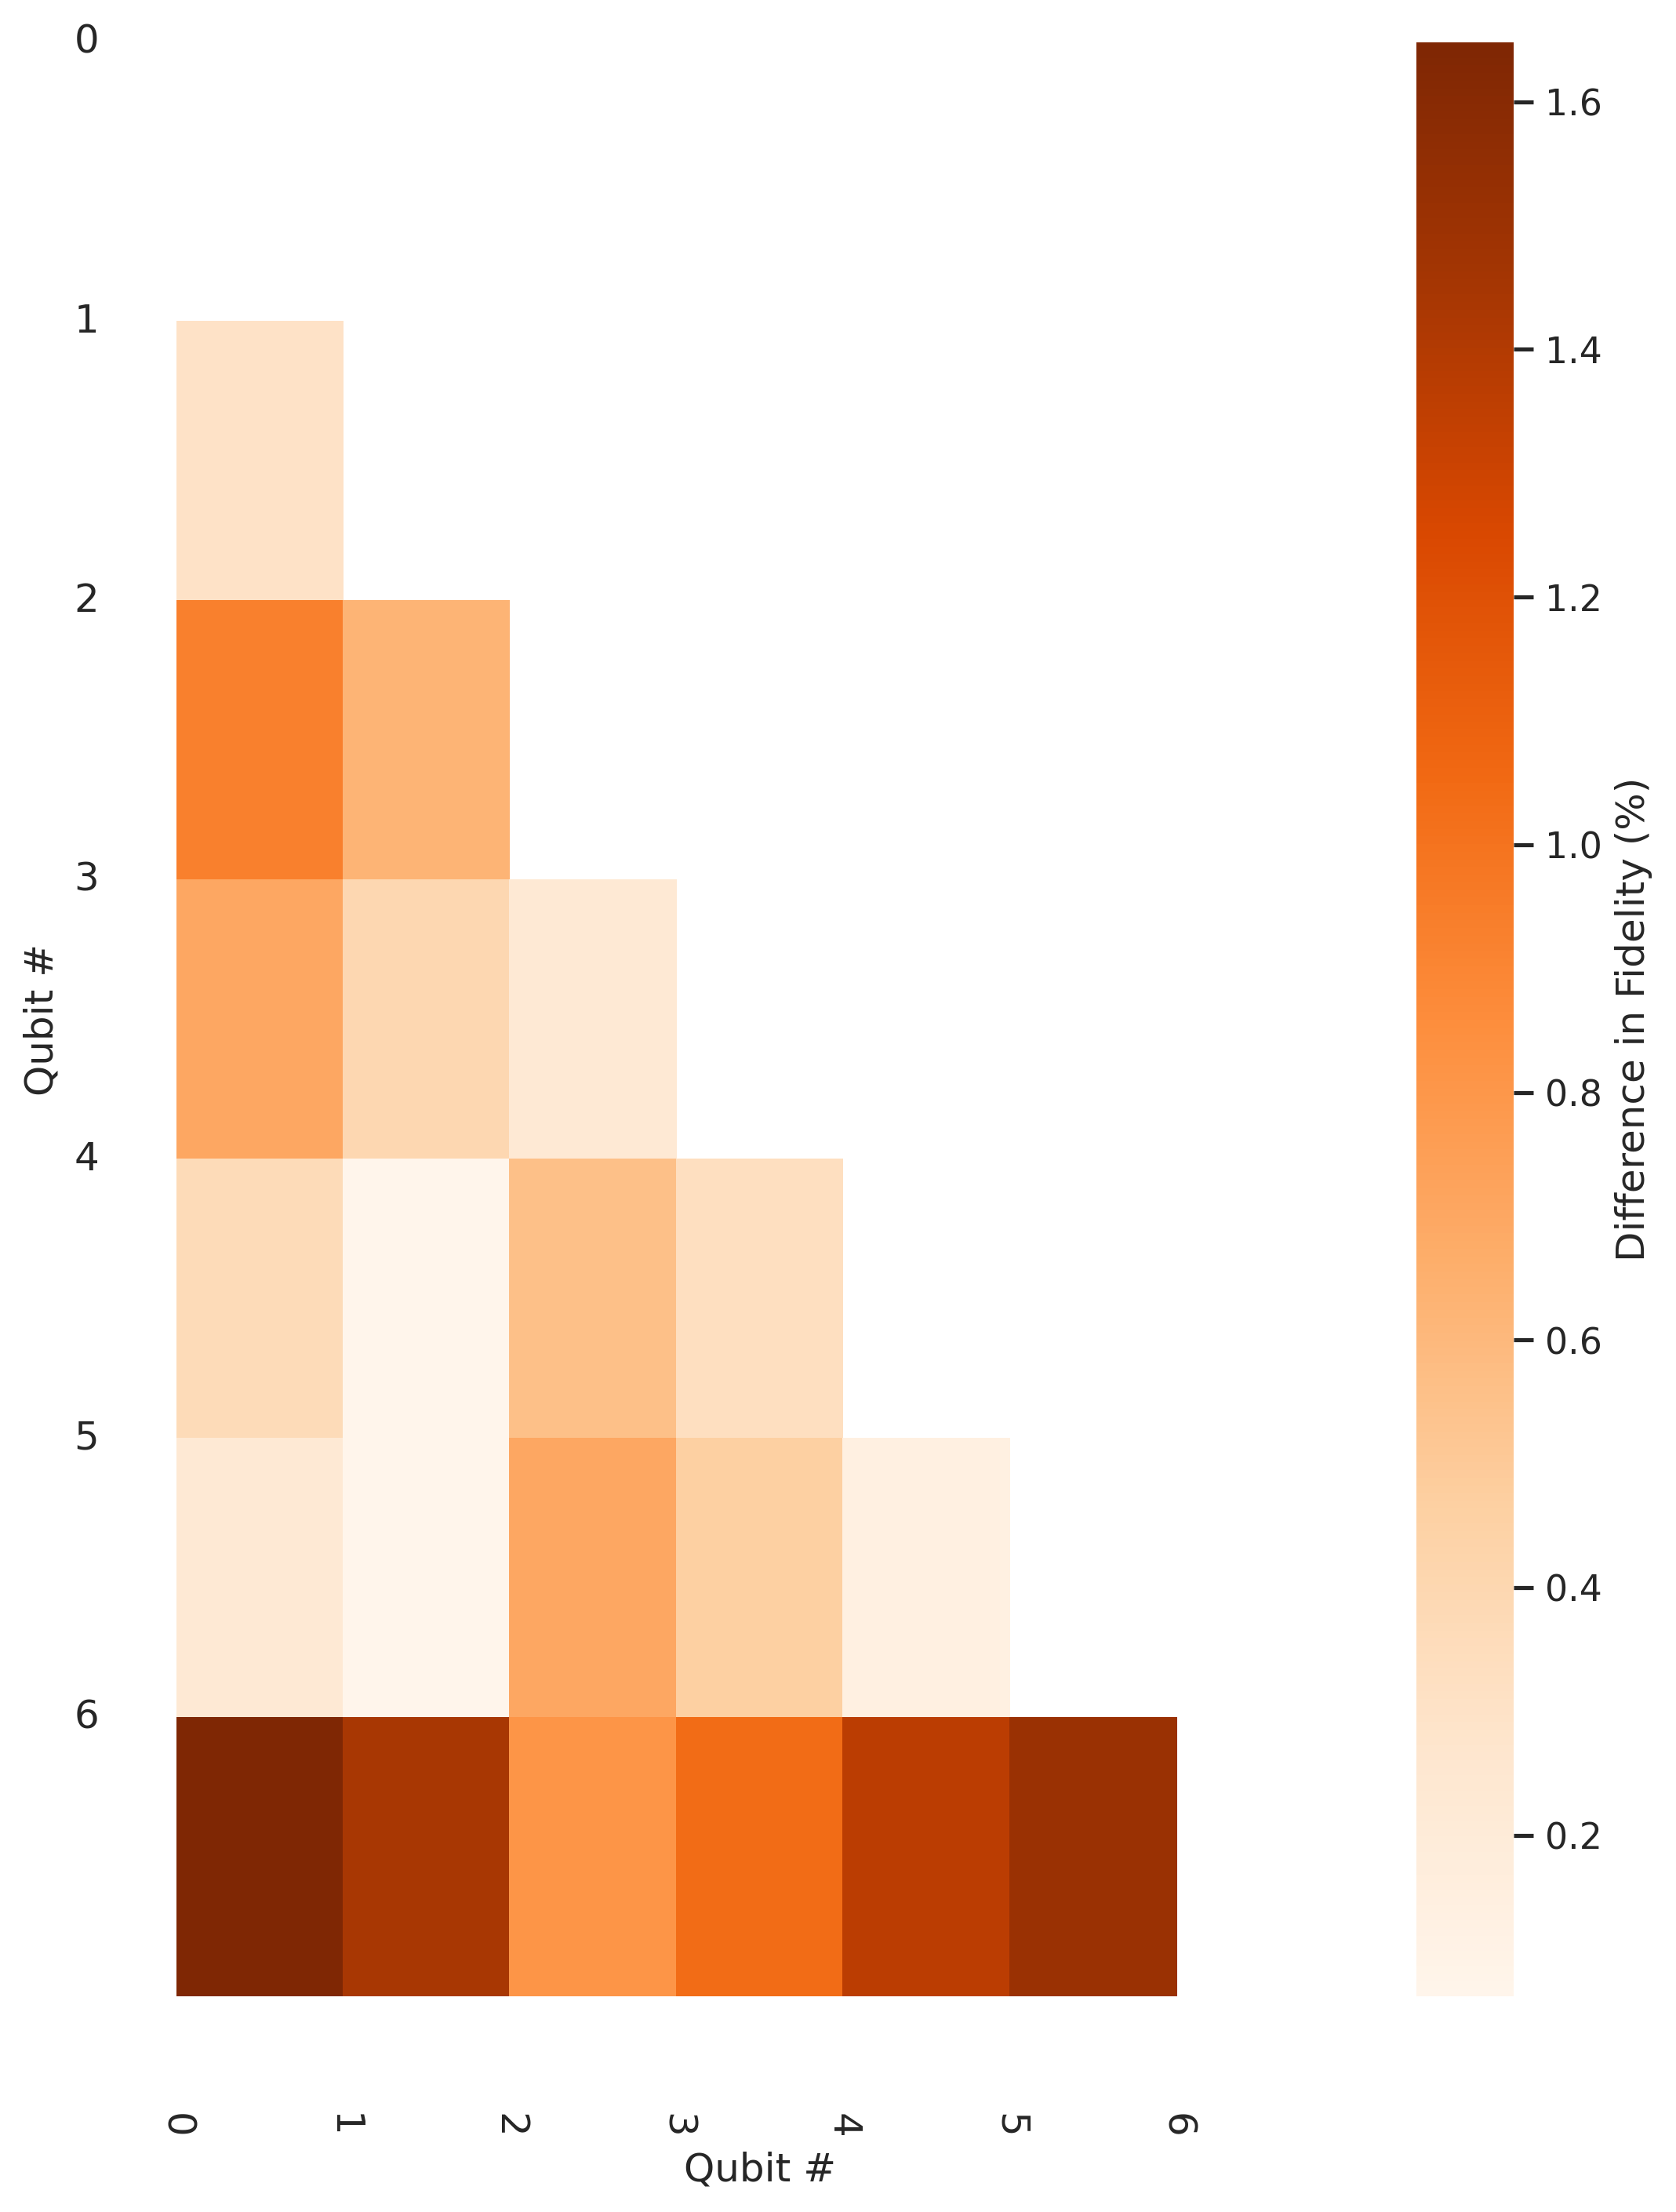
\includegraphics[height=0.8\textheight]{FI_raw_lattice.png}
\label{fig:FI_raw_lattice}
\caption{Characterizing the point-in-time variability of the initialization fidelity of the 127 qubits of \washington. Cell $[i,j]$ contains the difference between the initialization fidelity of register $i$ and that of register $j$ on March 8, 2022. High values (bad) imply high variability and are shaded by the darker end of the spectrum.}
\end{figure*}
%%%%%%%%%%%%%%%%%%%%%%%%%

%%%%%%%%%%%%%%%%%%%%%%%%%%
\begin{figure*} % for sub figures over two columns in 
\centering
\subfloat[Zero]{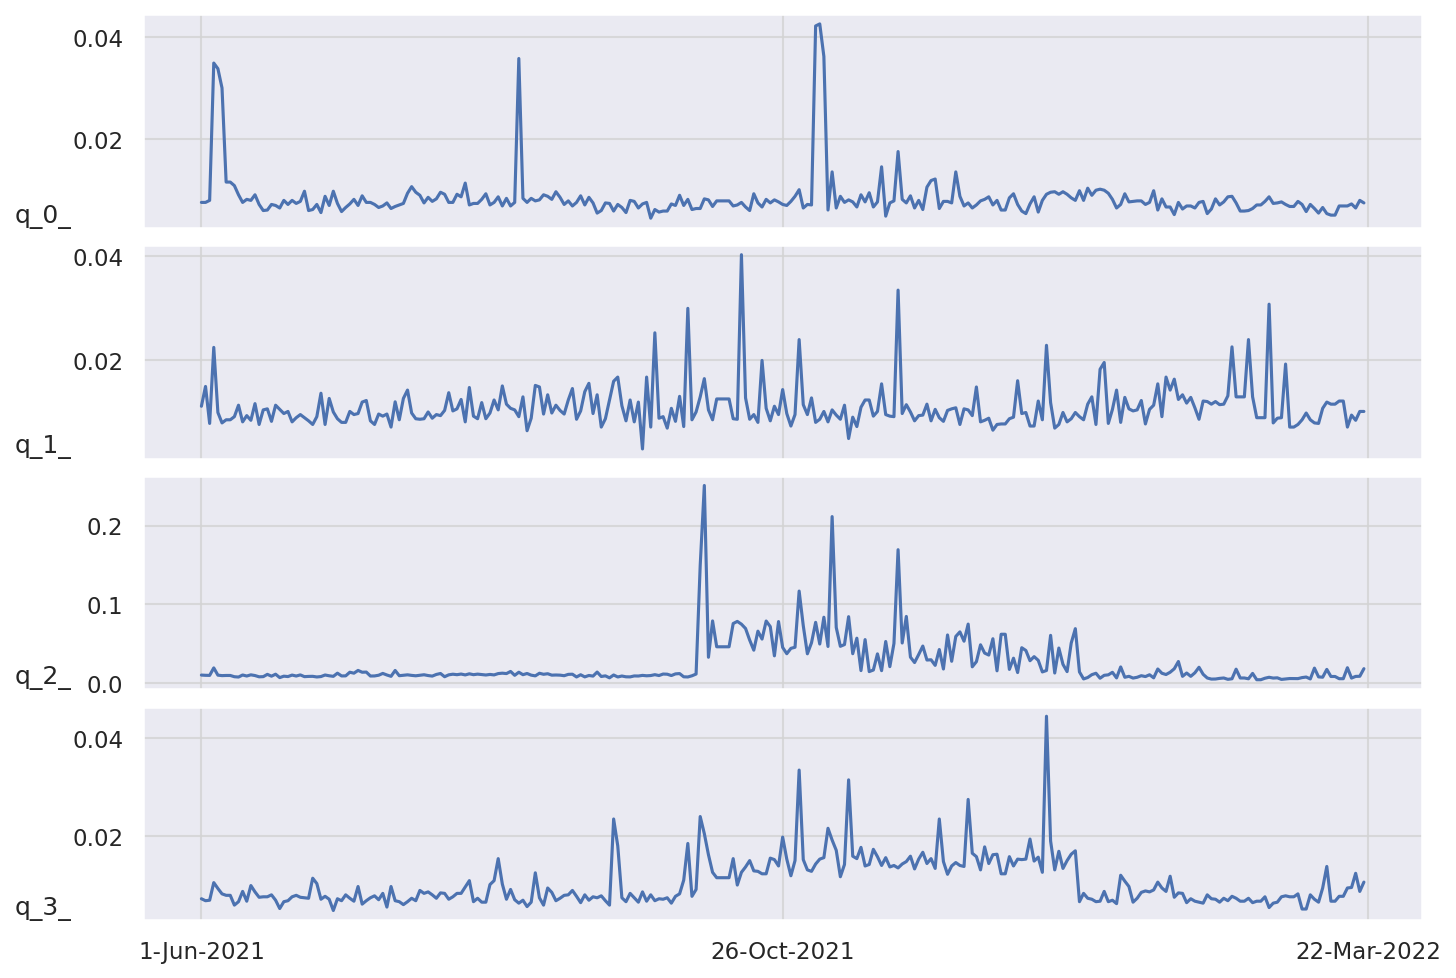
\includegraphics[width=0.64\columnwidth]{FI_raw_time_0.png}\label{fig:FI_raw_time_0}}
\hfil
\subfloat[One]{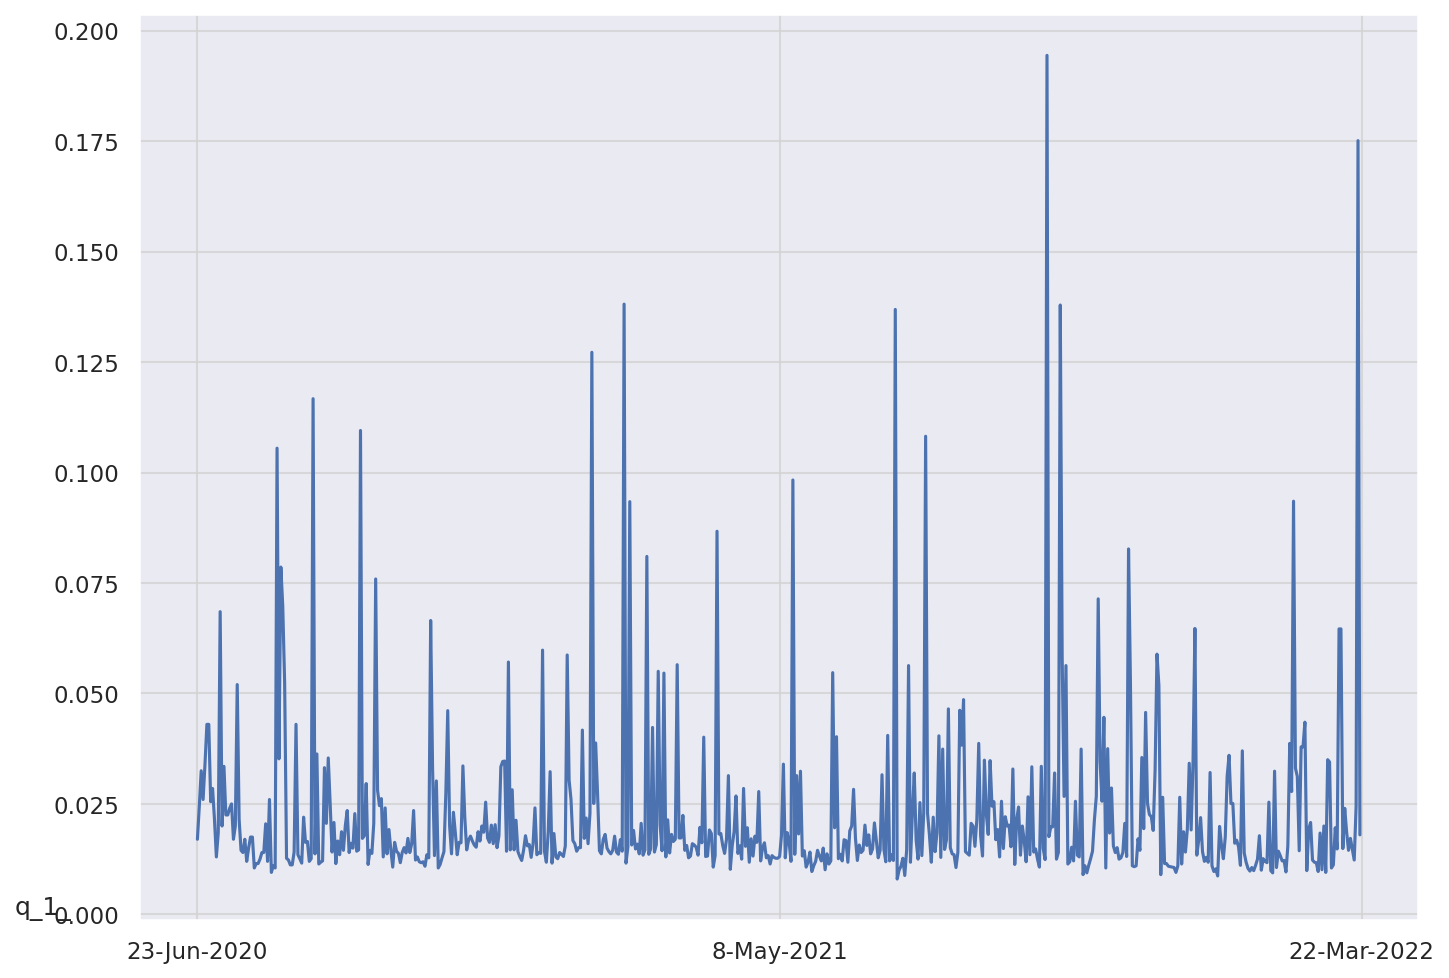
\includegraphics[width=0.64\columnwidth]{FI_raw_time_1.png}\label{fig:FI_raw_time_1}}

\subfloat[Two]{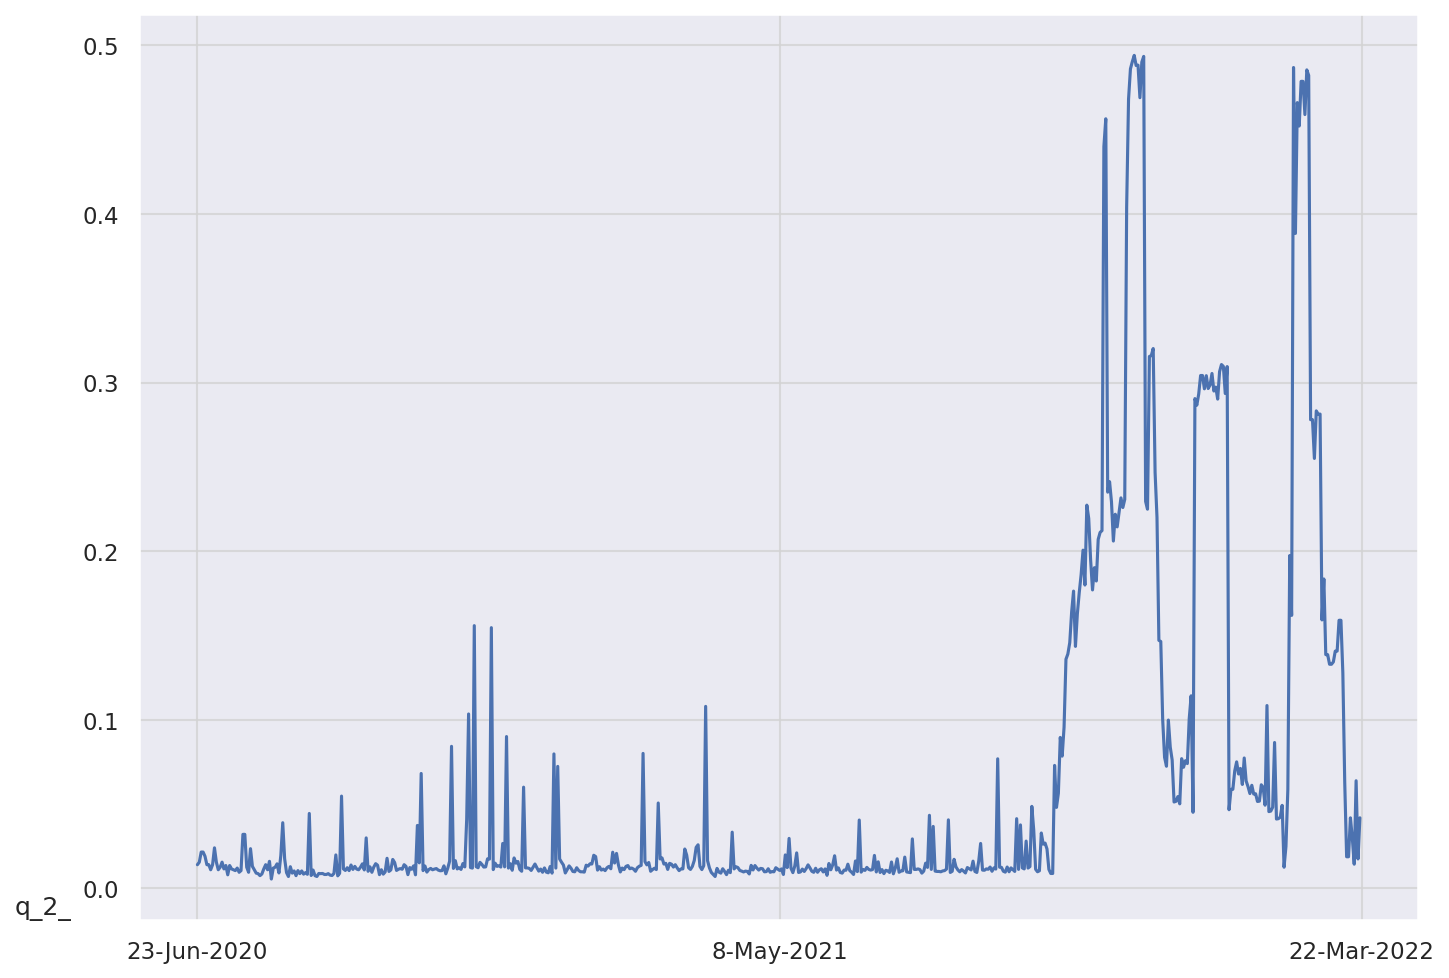
\includegraphics[width=0.64\columnwidth]{FI_raw_time_2.png}\label{fig:FI_raw_time_2}}
\hfil
\subfloat[Three]{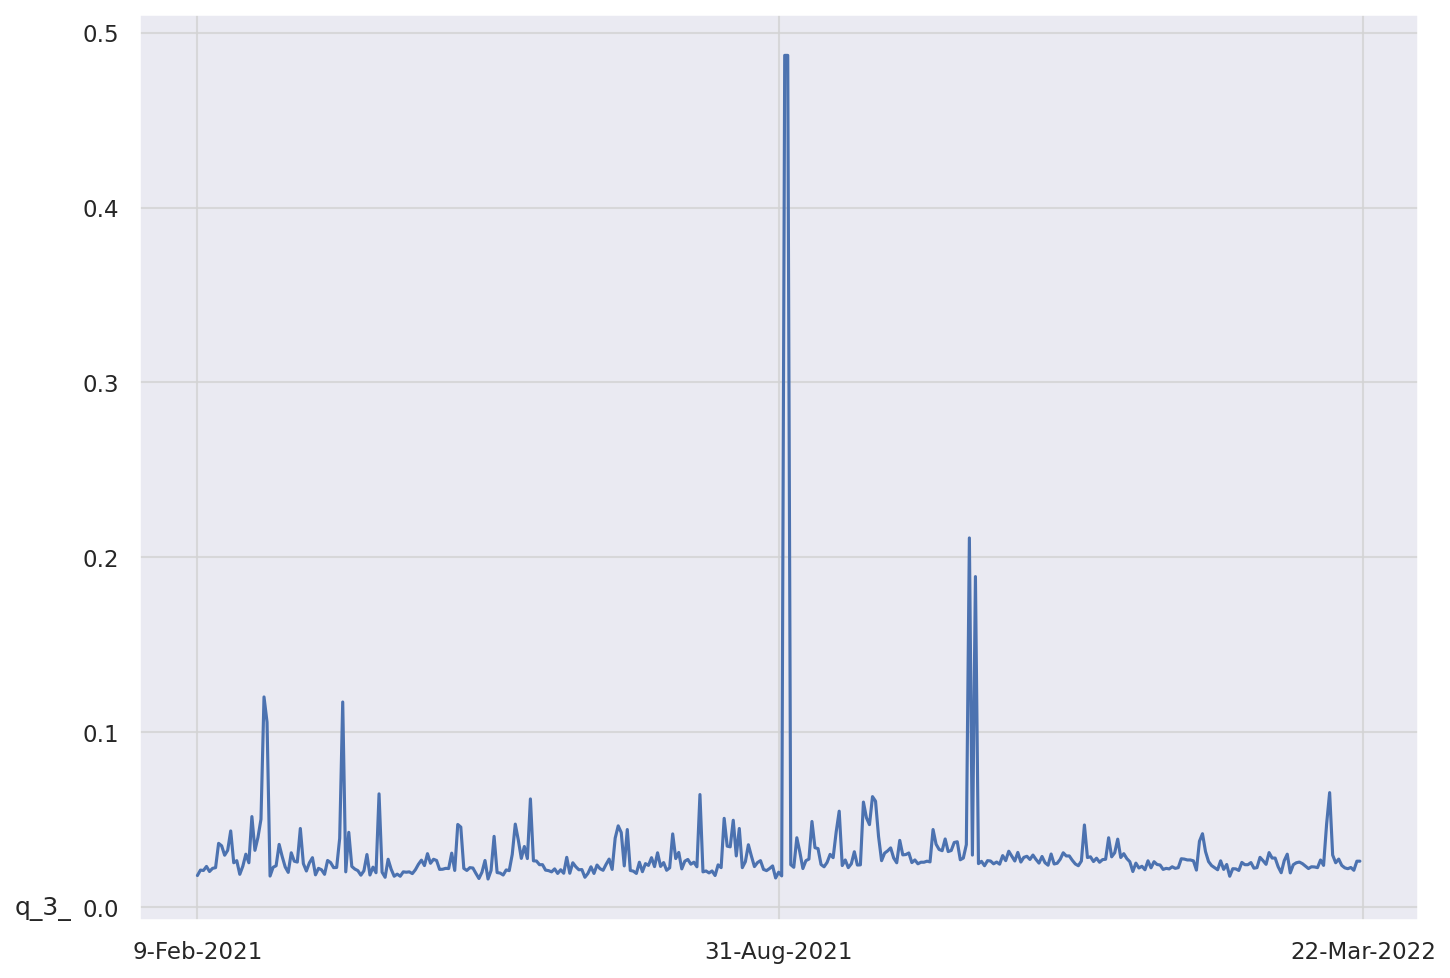
\includegraphics[width=0.64\columnwidth]{FI_raw_time_3.png}\label{fig:FI_raw_time_3}}

\subfloat[Four]{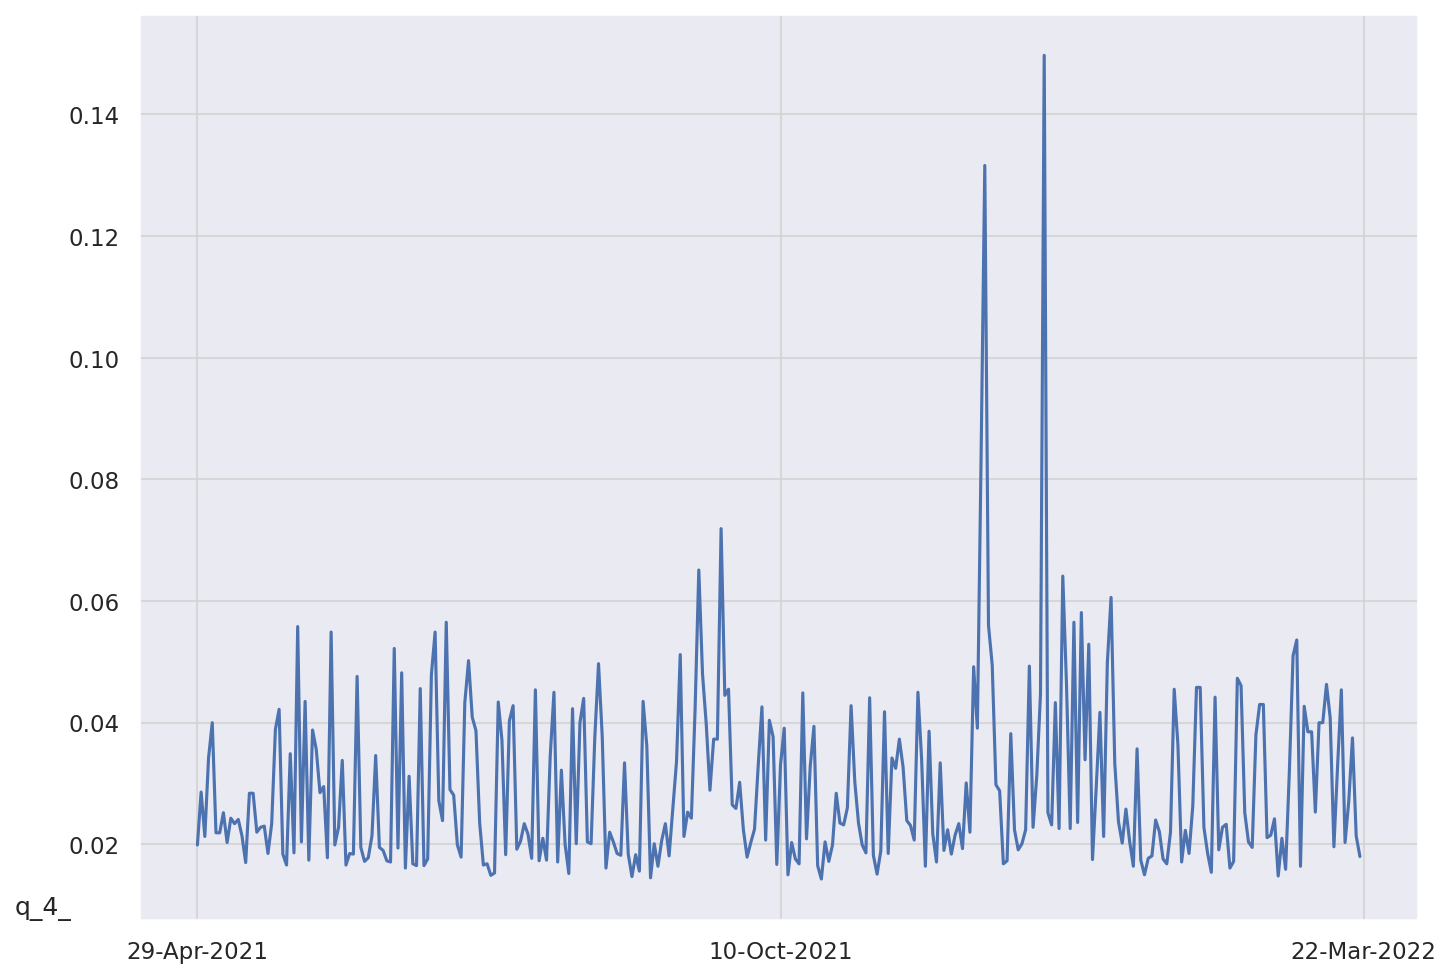
\includegraphics[width=0.64\columnwidth]{FI_raw_time_4.png}\label{fig:FI_raw_time_4}}
\hfil
\subfloat[Five]{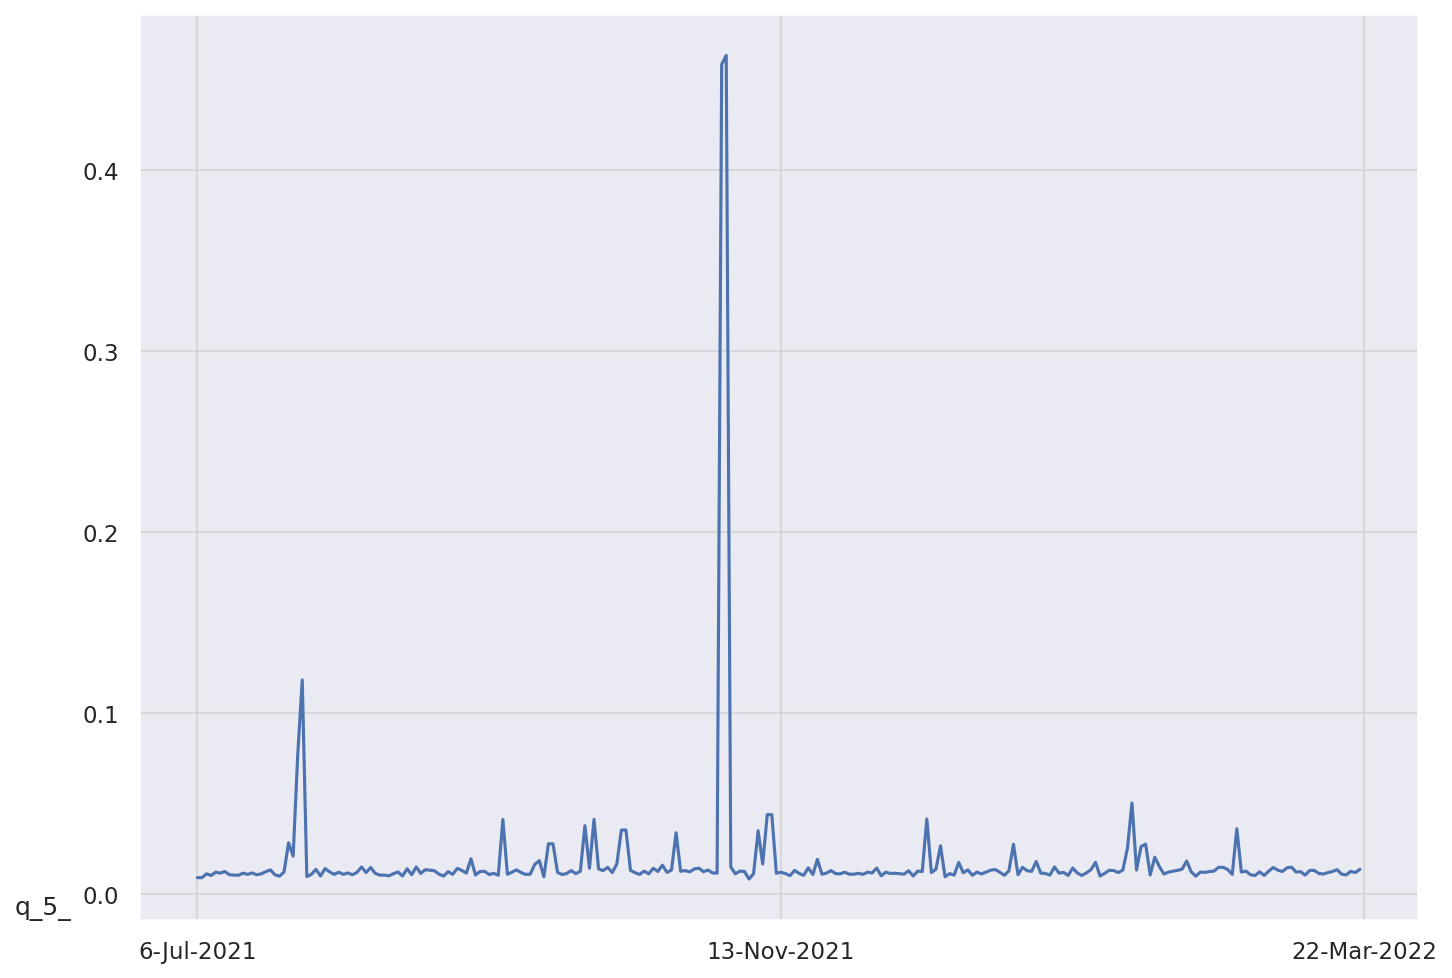
\includegraphics[width=0.64\columnwidth]{FI_raw_time_5.png}\label{fig:FI_raw_time_5}}

\subfloat[Six]{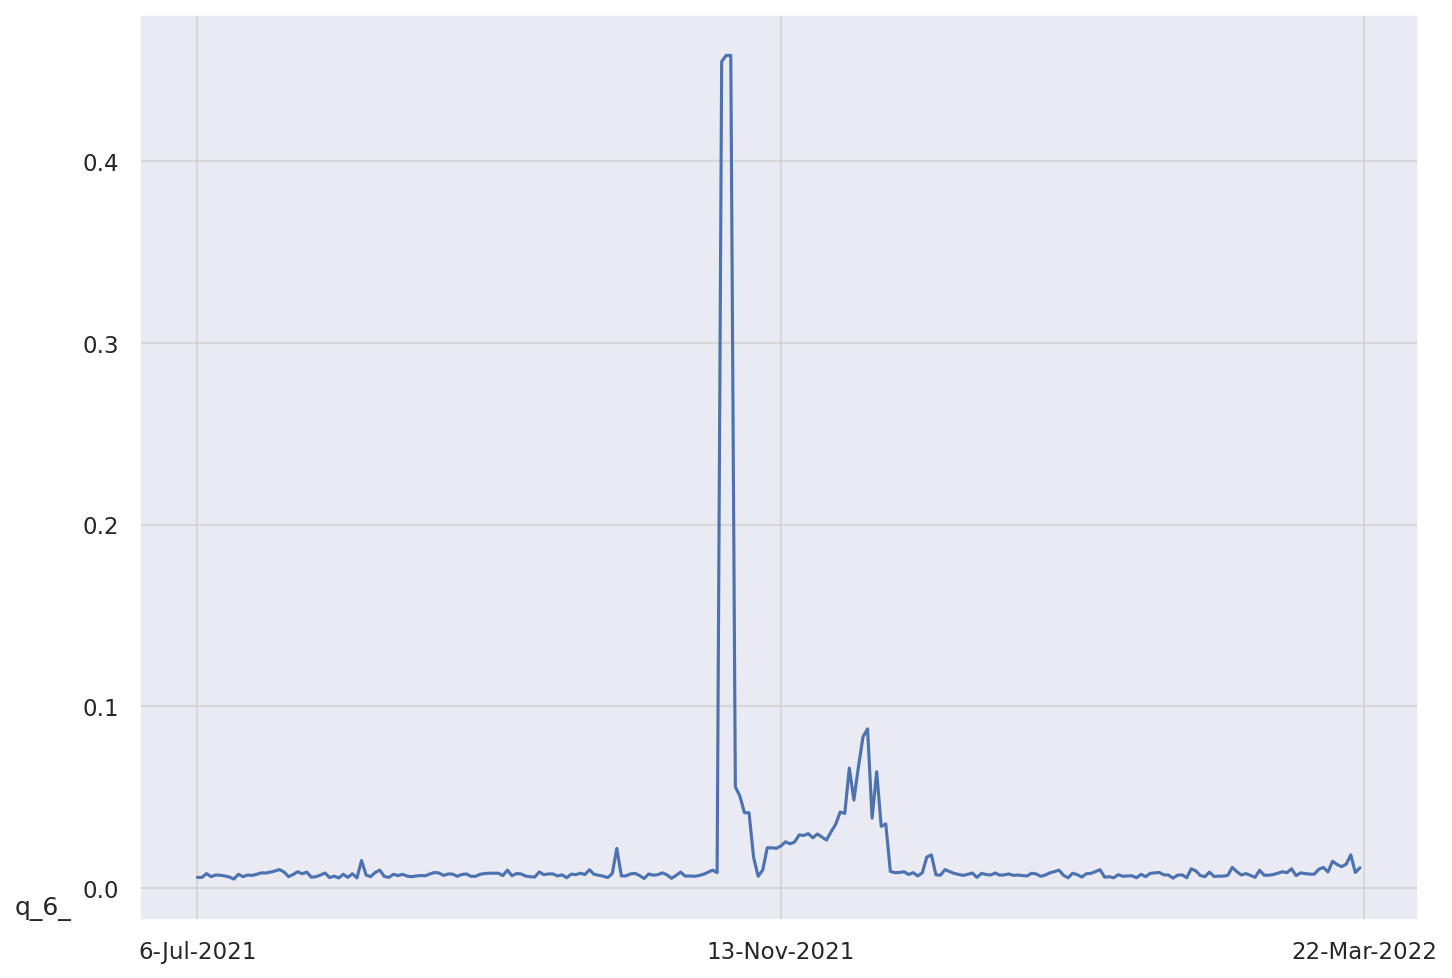
\includegraphics[width=0.64\columnwidth]{FI_raw_time_6.png}\label{fig:FI_raw_time_6}}
\hfil
\subfloat[Seven]{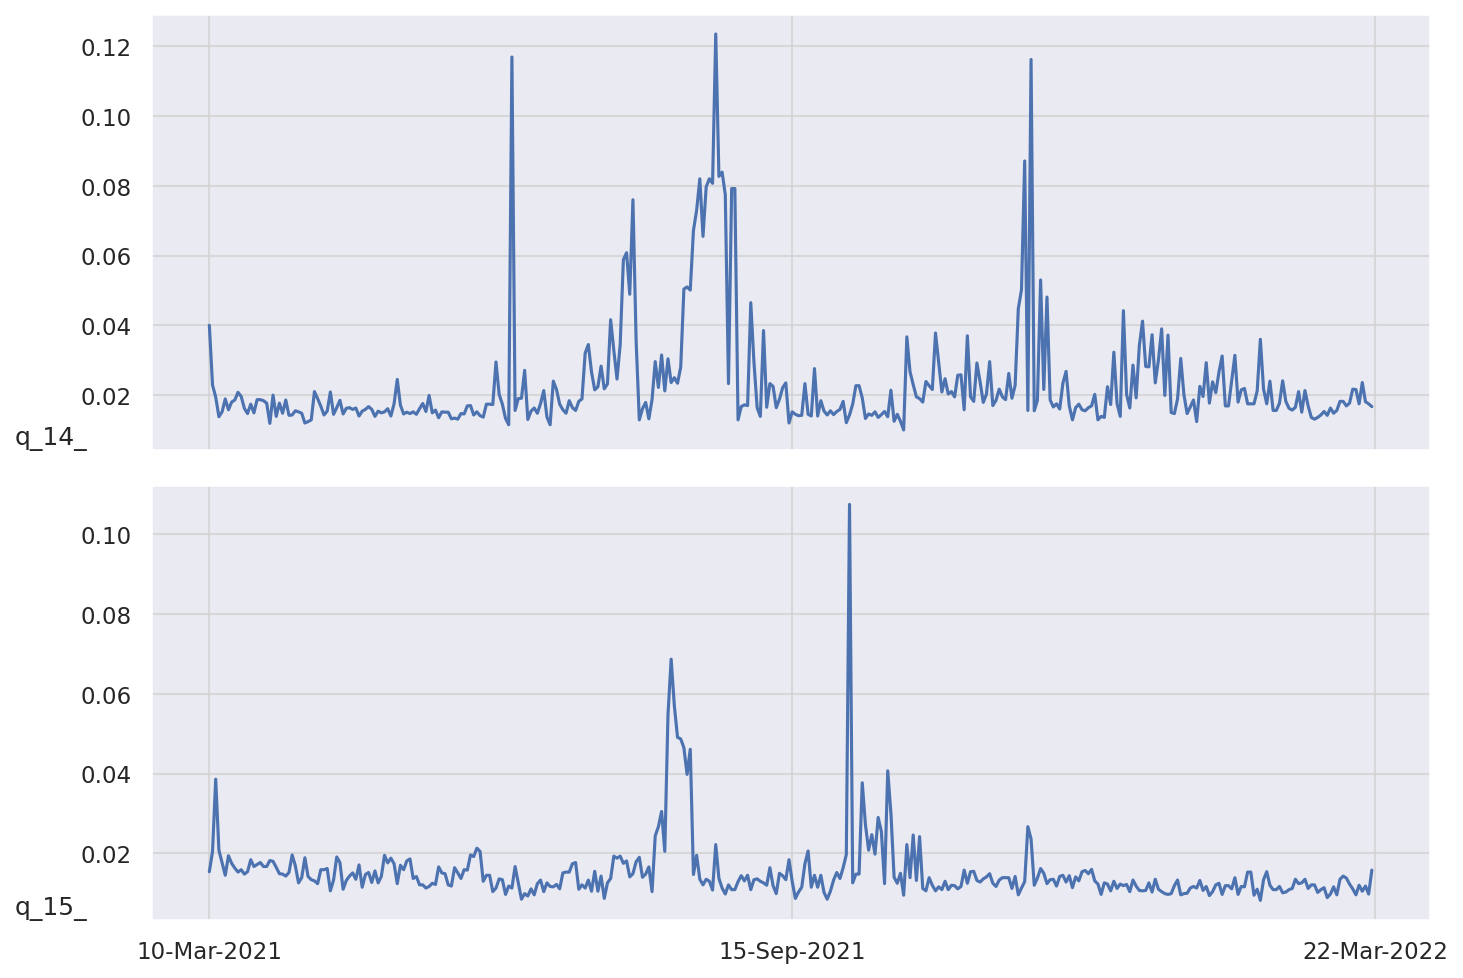
\includegraphics[width=0.64\columnwidth]{FI_raw_time_7.png}\label{fig:FI_raw_time_7}}

\caption{Characterizing the across-time variability the initialization fidelity of the 127 qubits of \washington. The data in the 8 plots shown above cover all the 127 qubits for the period 9 Dec, 2021 (when \washington was commissioned) to 8 Mar, 2022 (date of writing). The vertical axis represents the initialization fidelity $\in [0, 1]$ expressed as percentage. The horizontal axis represents time.}
% of the \protect\subref{fig:yorktown} \yorktown and \protect\subref{fig:toronto} \toronto devices produced by IBM. Circles denote register elements and edges denote connectivity of 2-qubit operations.}
\label{fig:tbd}
\end{figure*}
%%%%%%%%%%%%%%%%%%%%%%%%%%

\subsection*{Gate Fidelity}
%%%%%%%%%%%%%%%%%%%%%%%%%
\begin{figure*} % for sub figures over two columns in 
\centering
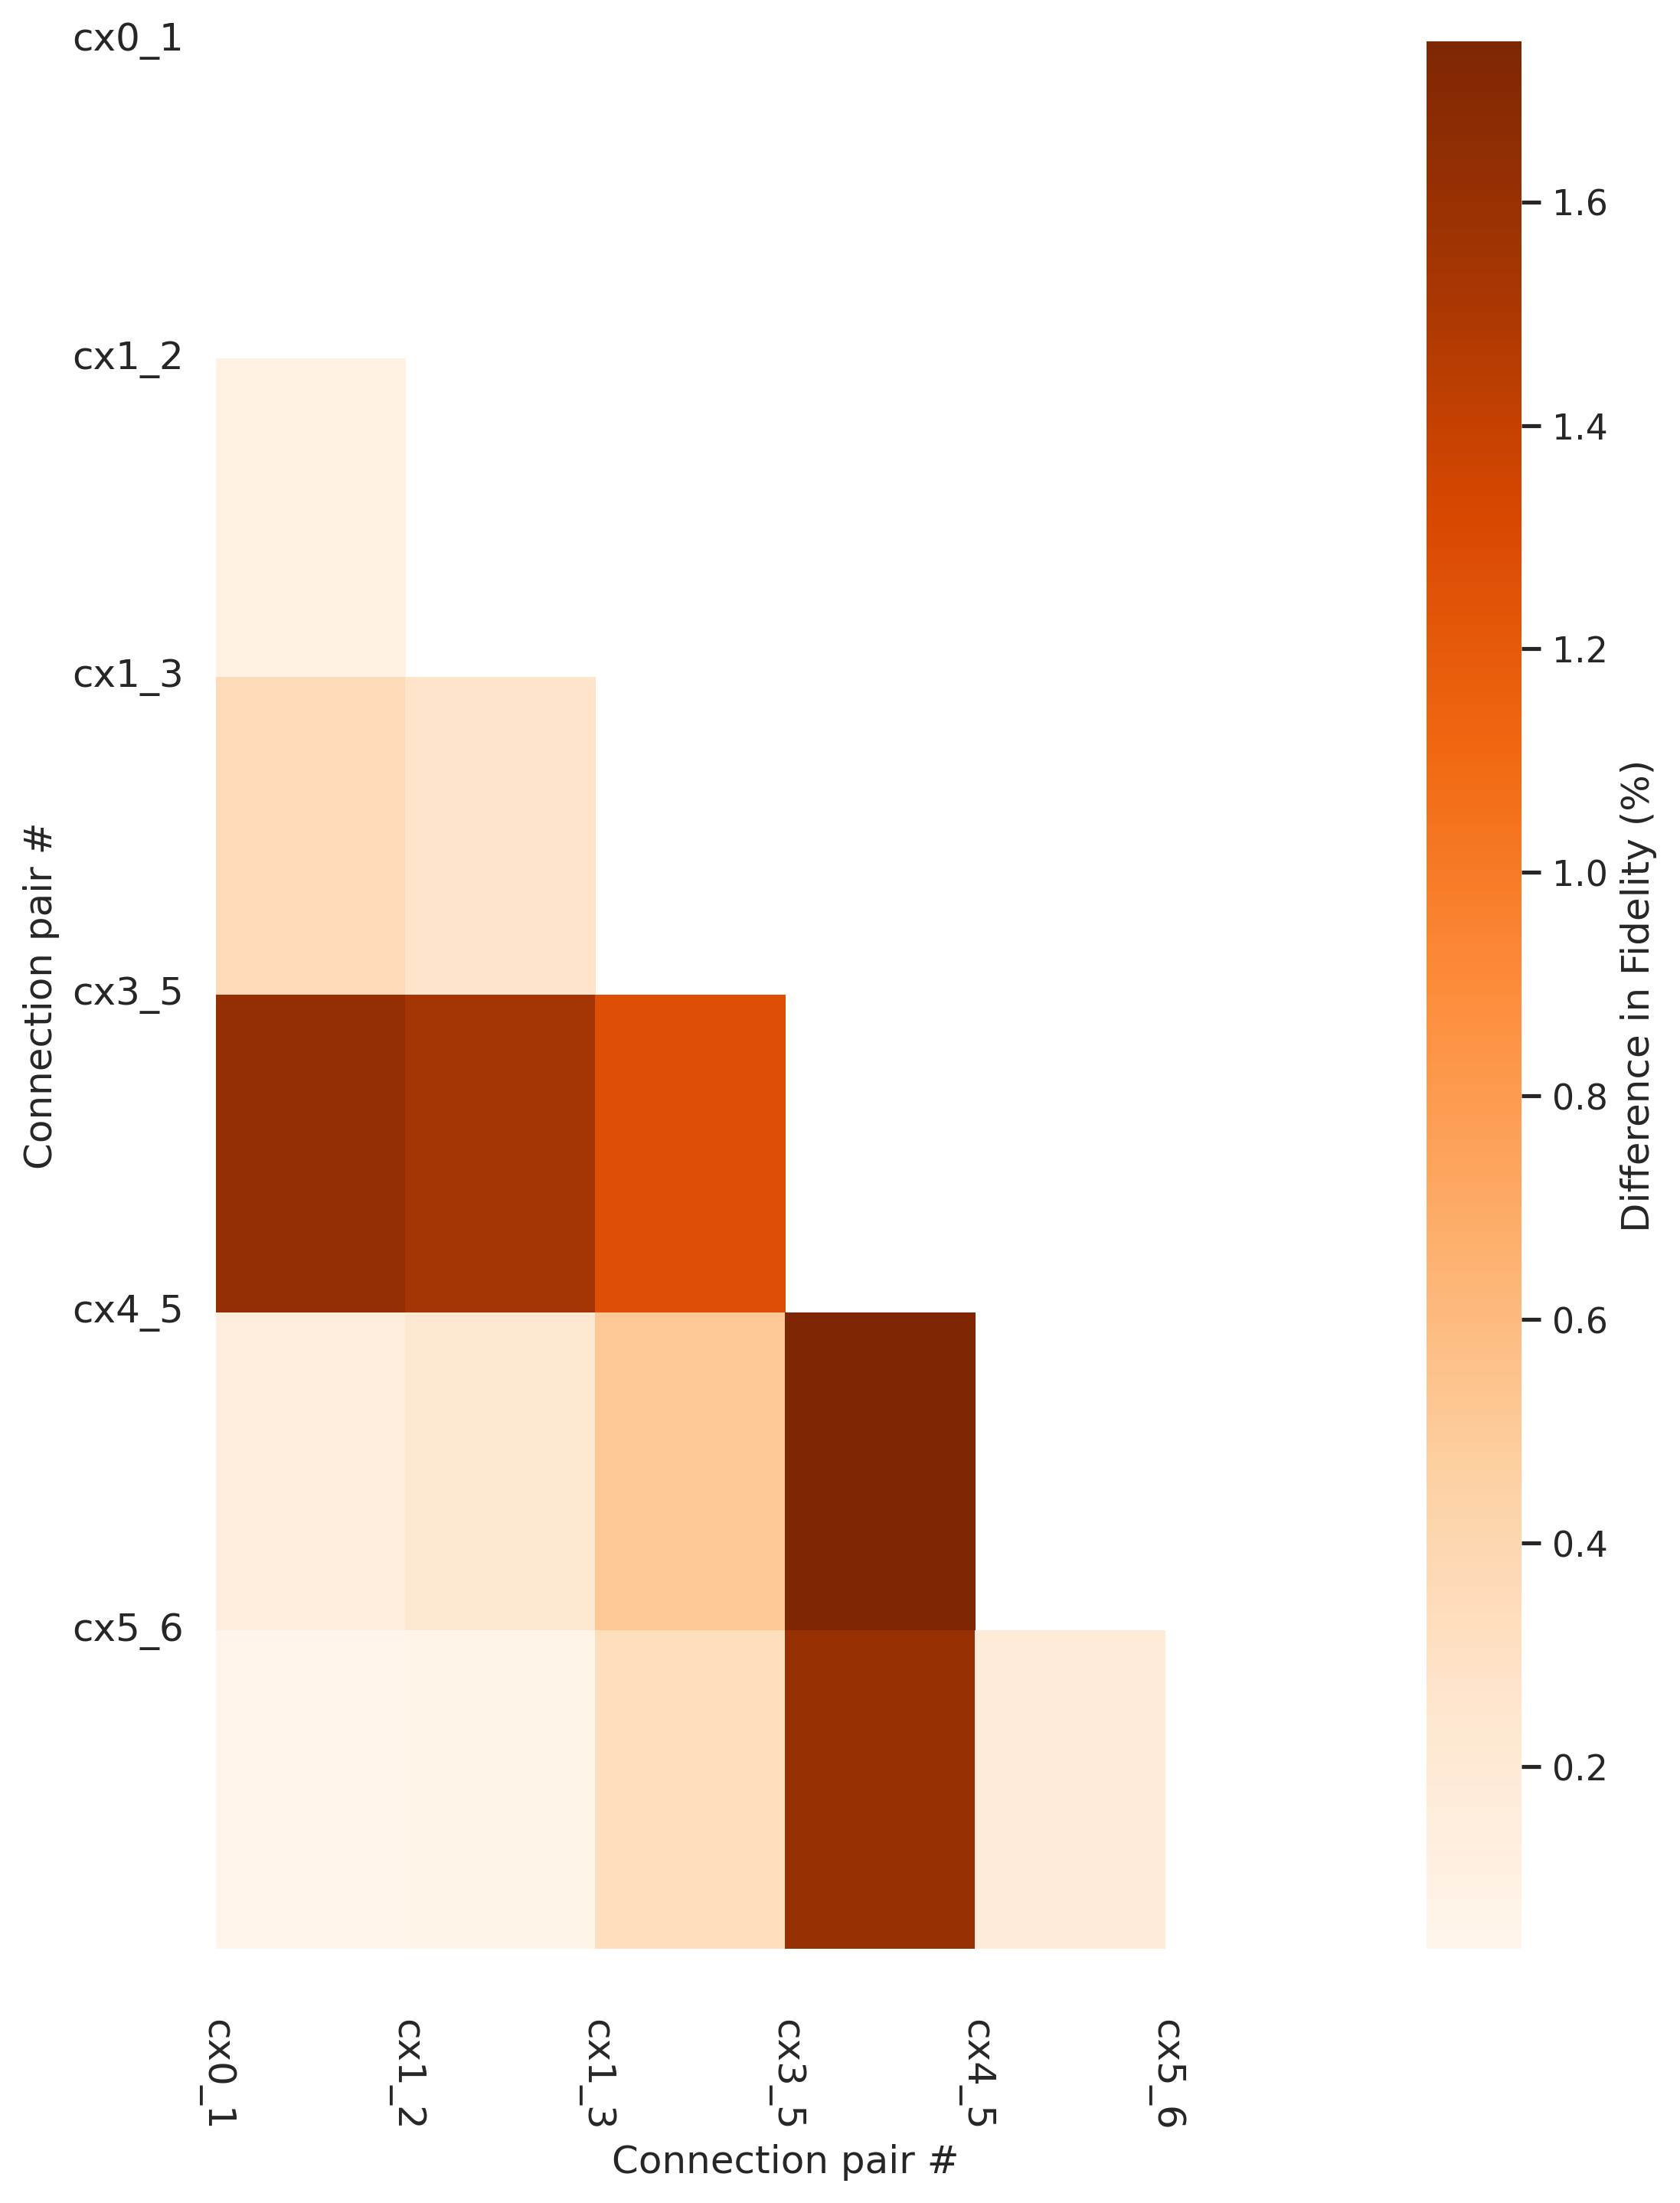
\includegraphics[height=0.8\textheight]{FG_raw_lattice.png}
\label{fig:FG_raw_lattice}
\caption{Characterizing the point-in-time variability of the CNOT fidelity of the permitted connections of \washington. Each cell contains the difference between the gate fidelities of different register pairs on March 8, 2022. High values (bad) imply high variability and are shaded by the darker end of the spectrum.}
\end{figure*}
%%%%%%%%%%%%%%%%%%%%%%%%%

%%%%%%%%%%%%%%%%%%%%%%%%%%
\begin{figure*} % for sub figures over two columns in 
\centering
\subfloat[Zero]{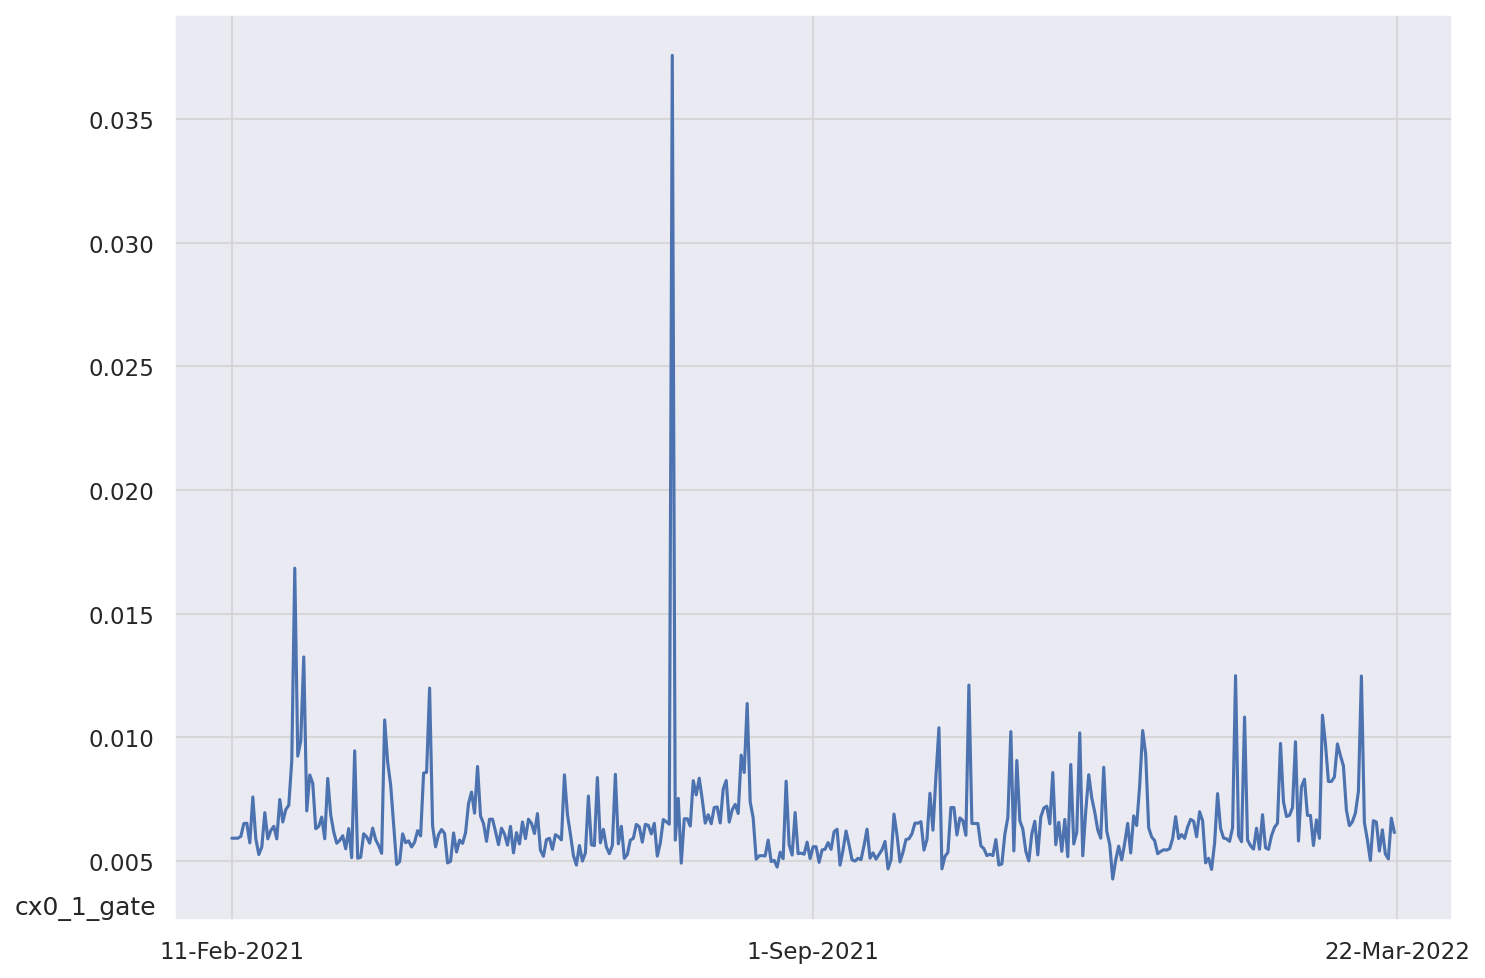
\includegraphics[width=0.64\columnwidth]{FG_raw_time_0.png}\label{fig:FG_raw_time_0}}
\hfil
\subfloat[One]{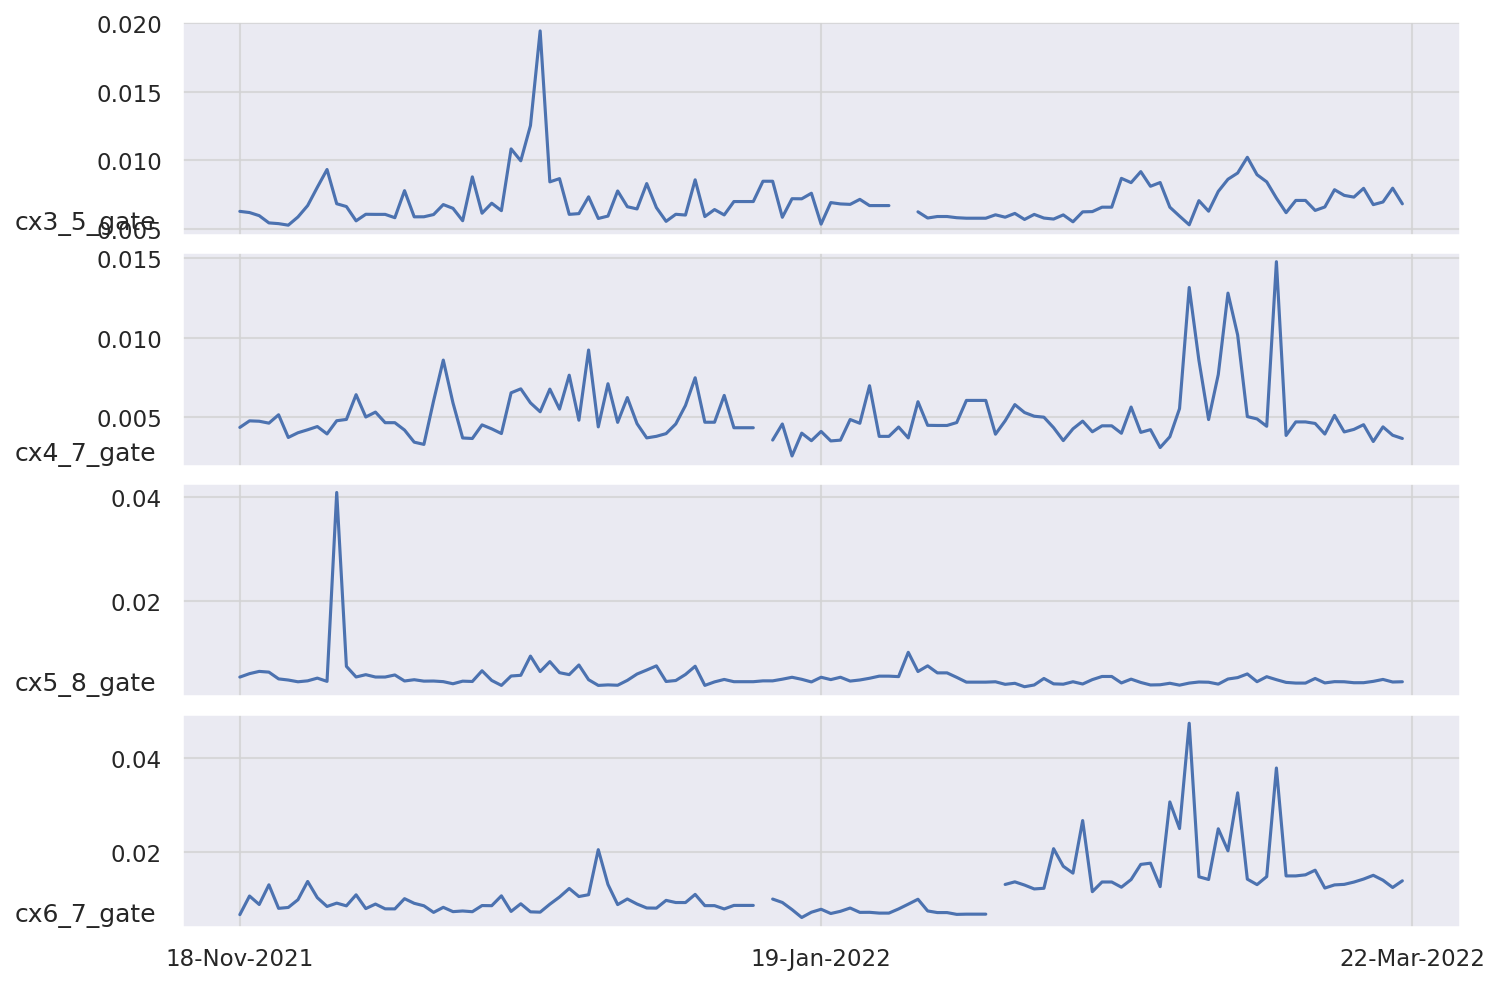
\includegraphics[width=0.64\columnwidth]{FG_raw_time_1.png}\label{fig:FG_raw_time_1}}

\subfloat[Two]{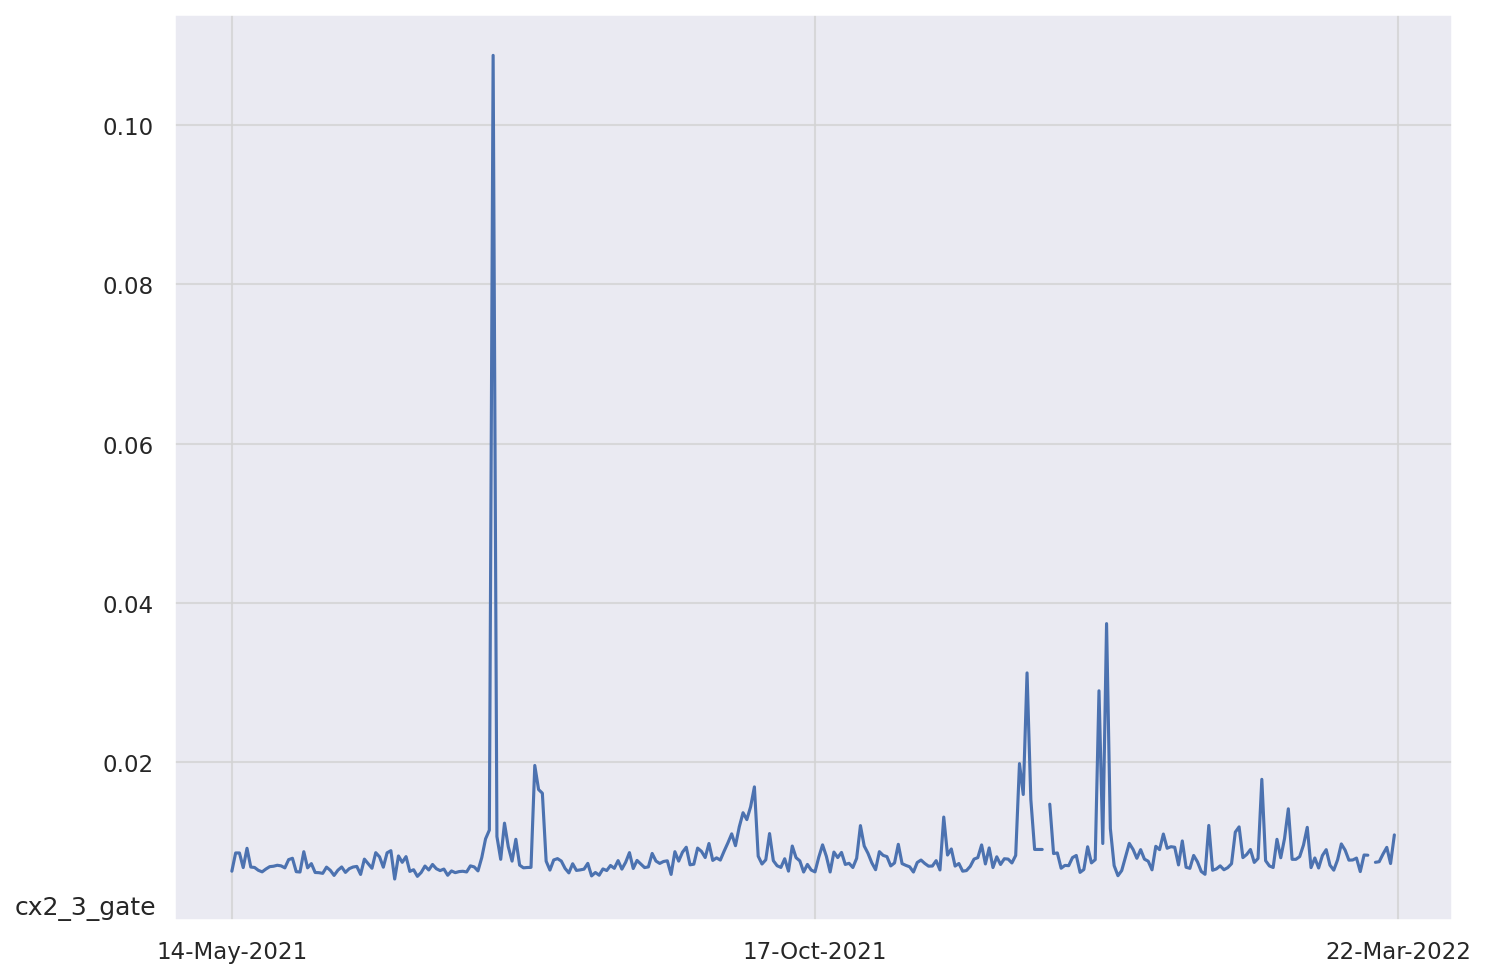
\includegraphics[width=0.64\columnwidth]{FG_raw_time_2.png}\label{fig:FG_raw_time_2}}
\hfil
\subfloat[Three]{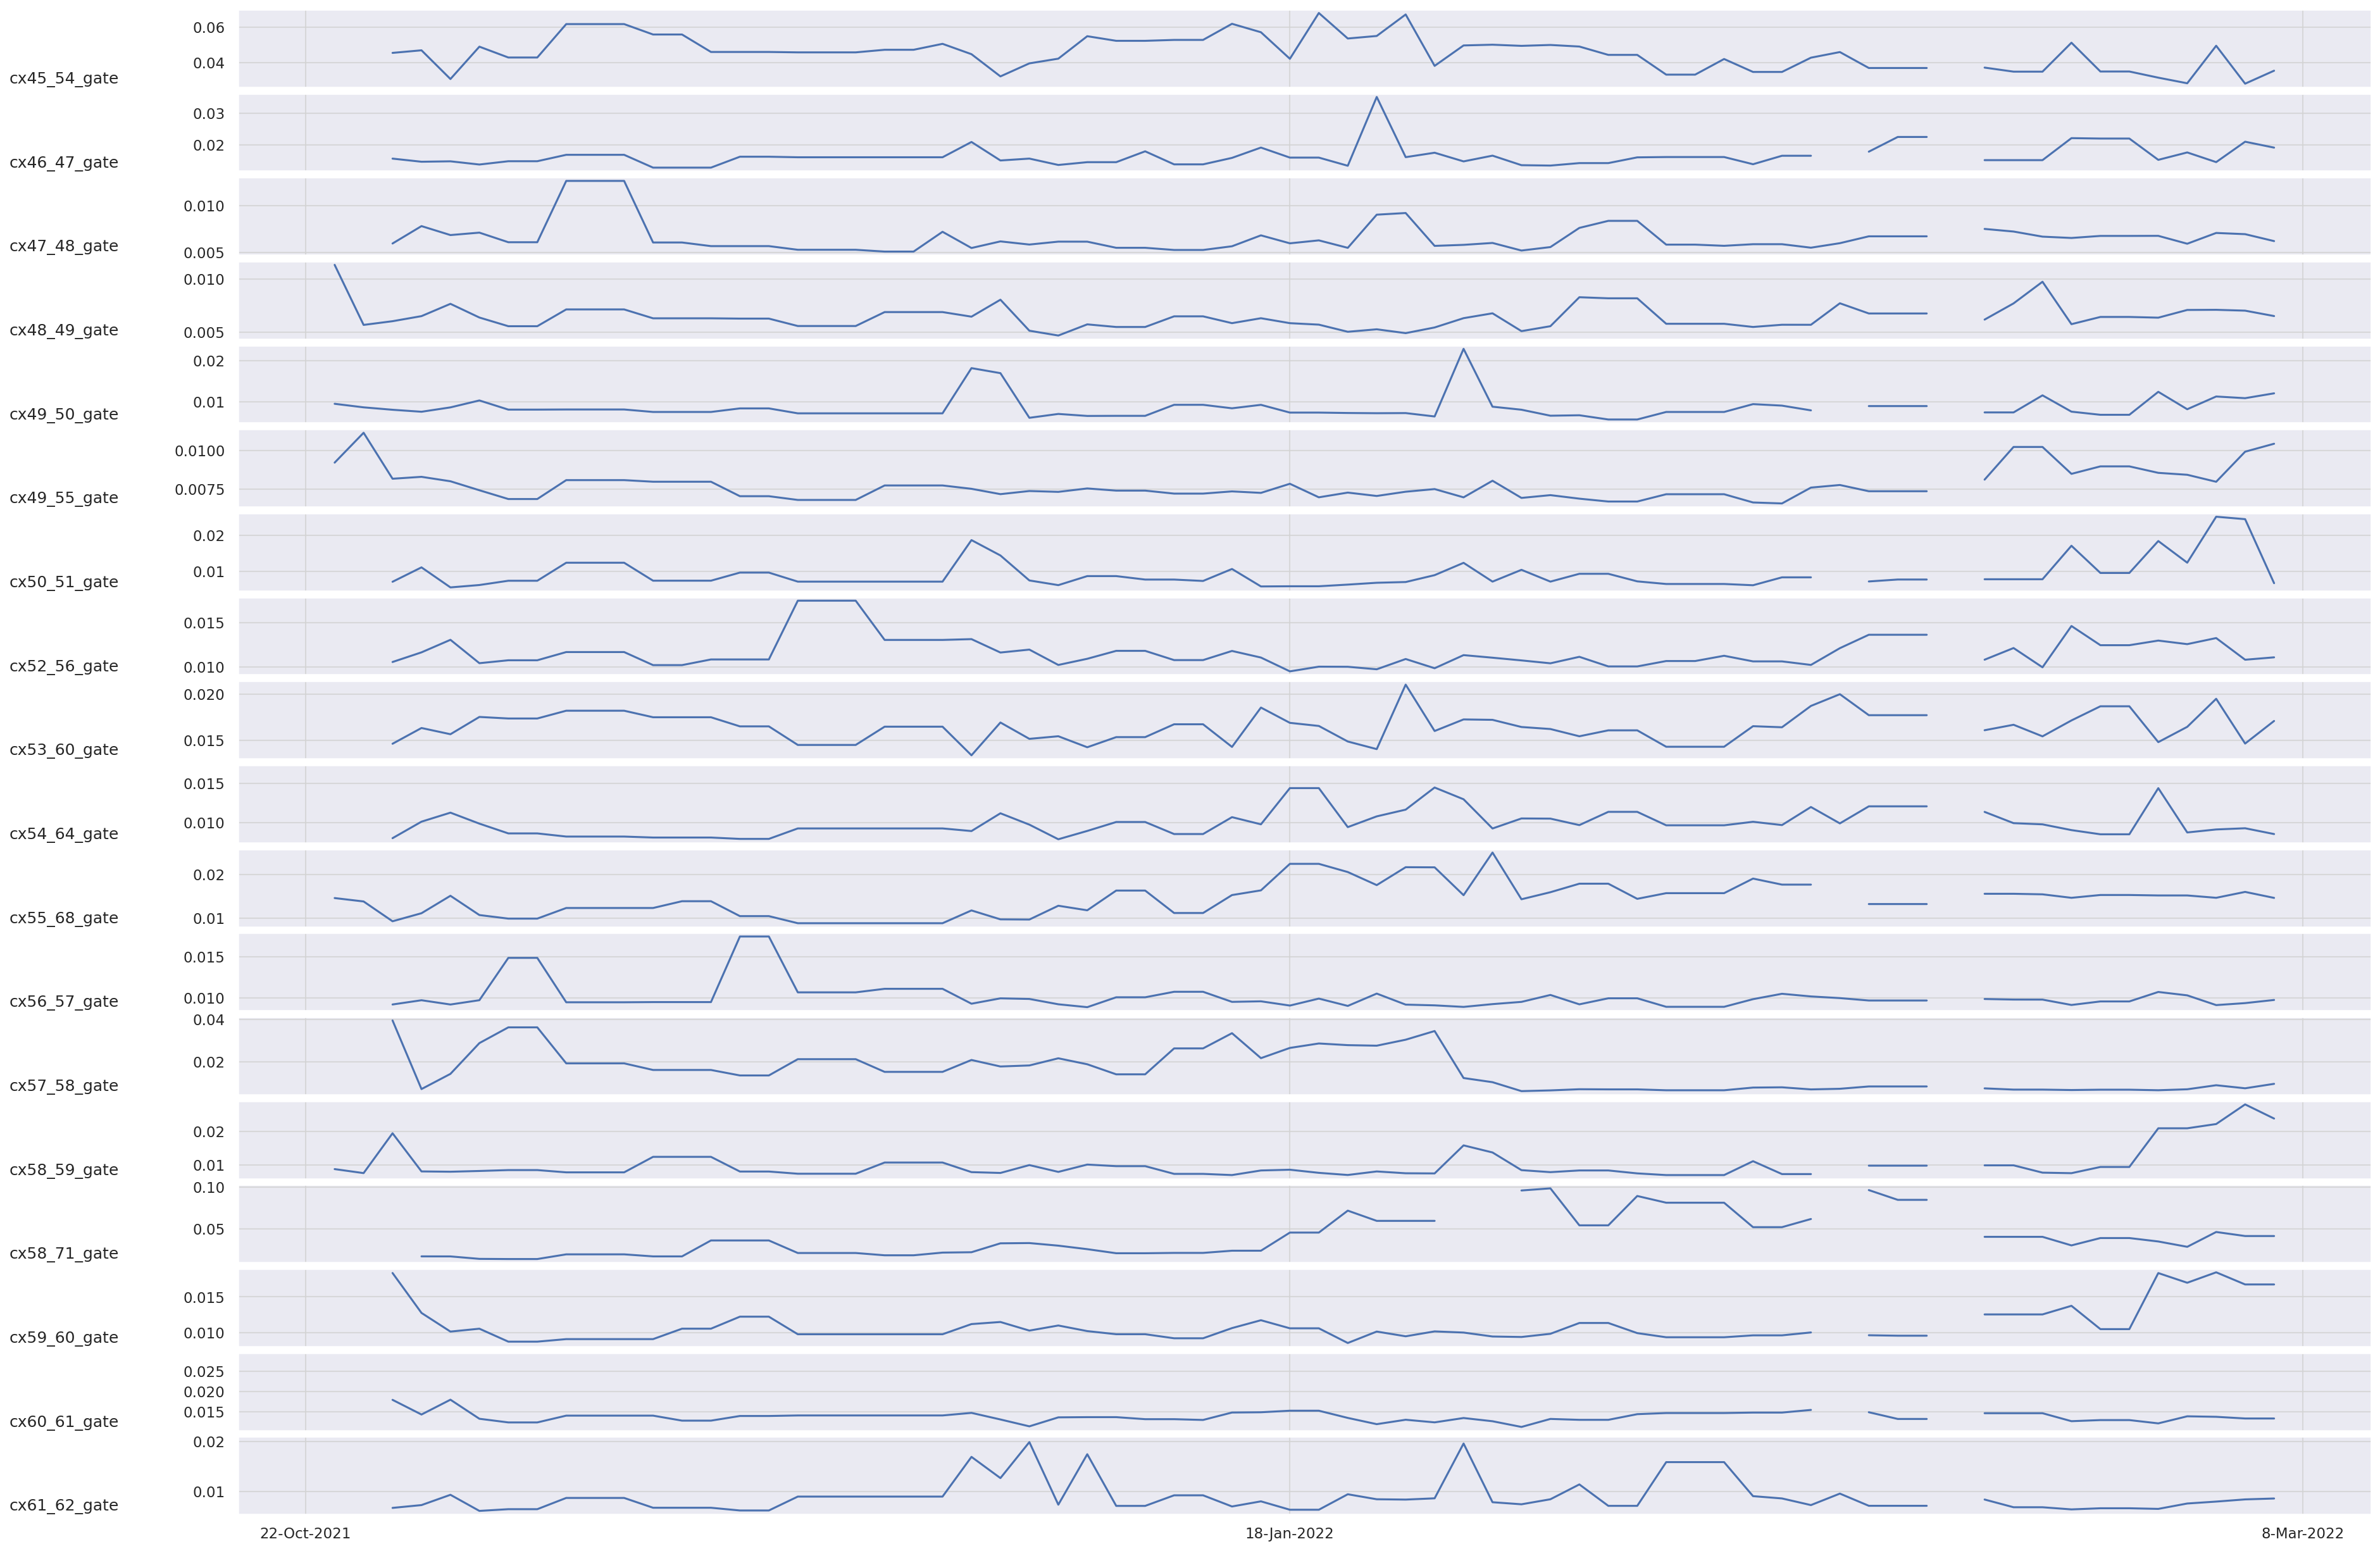
\includegraphics[width=0.64\columnwidth]{FG_raw_time_3.png}\label{fig:FG_raw_time_3}}

\subfloat[Four]{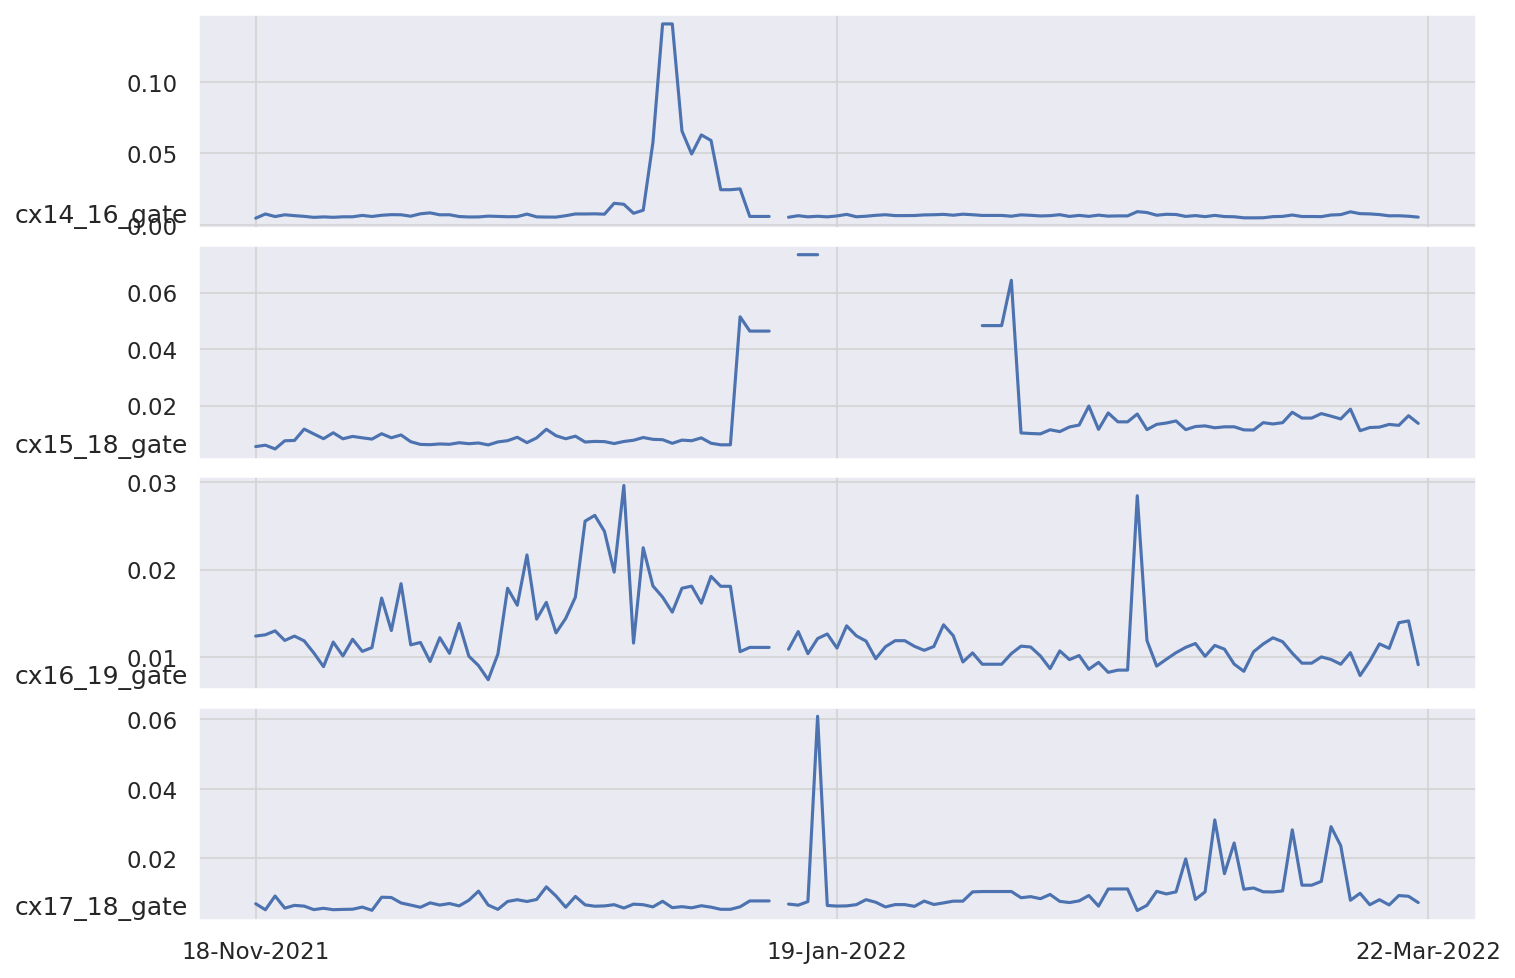
\includegraphics[width=0.64\columnwidth]{FG_raw_time_4.png}\label{fig:FG_raw_time_4}}
\hfil
\subfloat[Five]{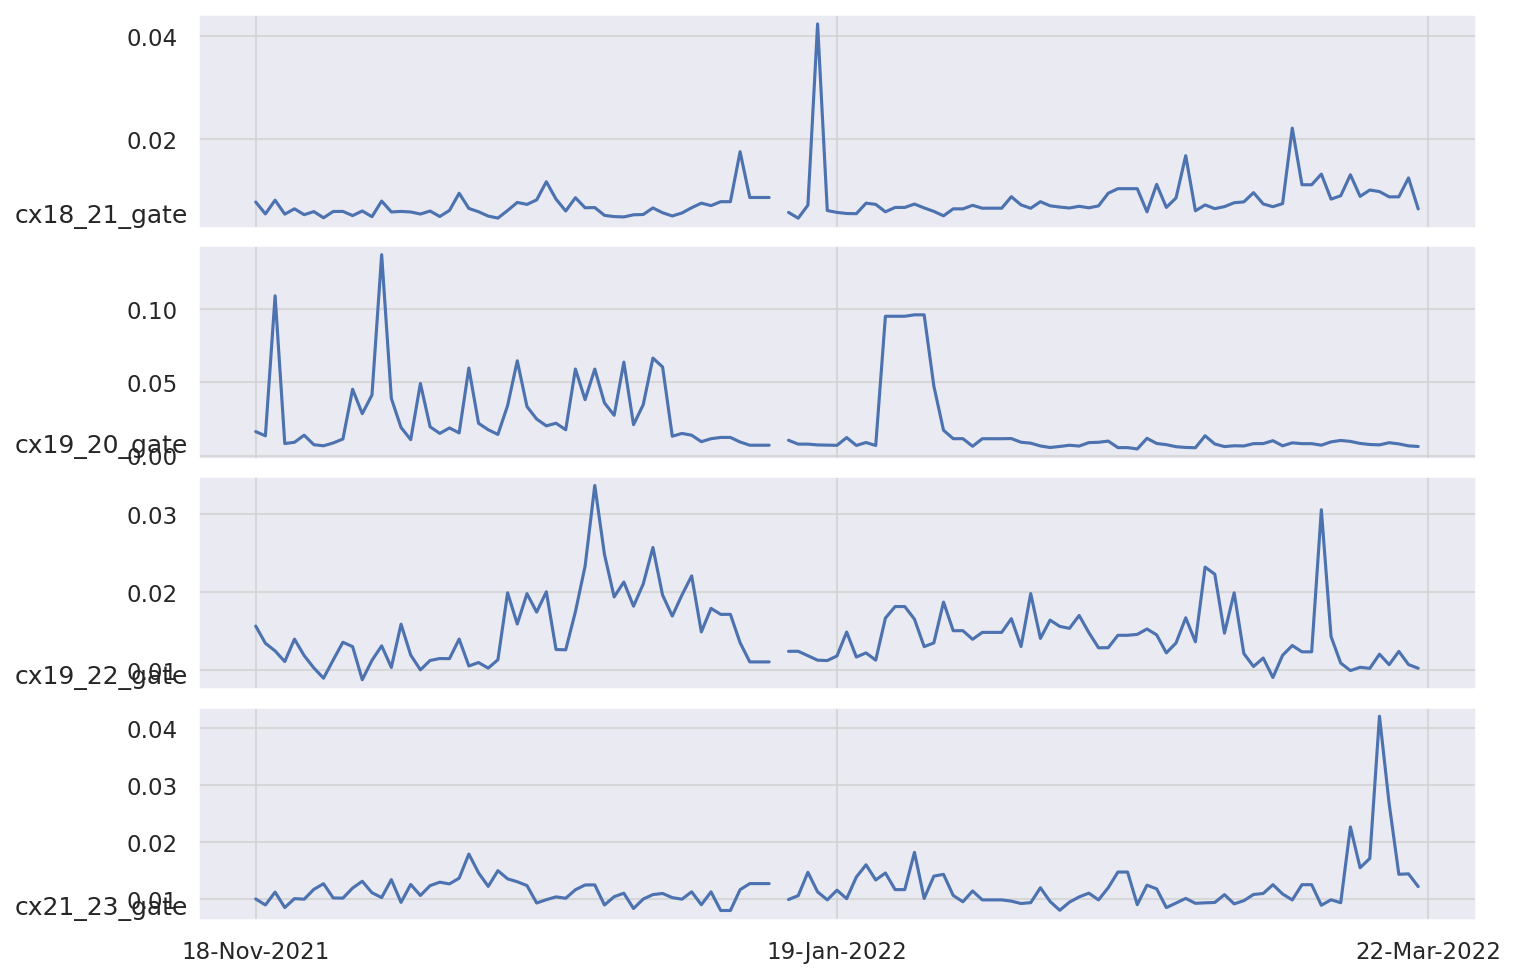
\includegraphics[width=0.64\columnwidth]{FG_raw_time_5.png}\label{fig:FG_raw_time_5}}

\subfloat[Six]{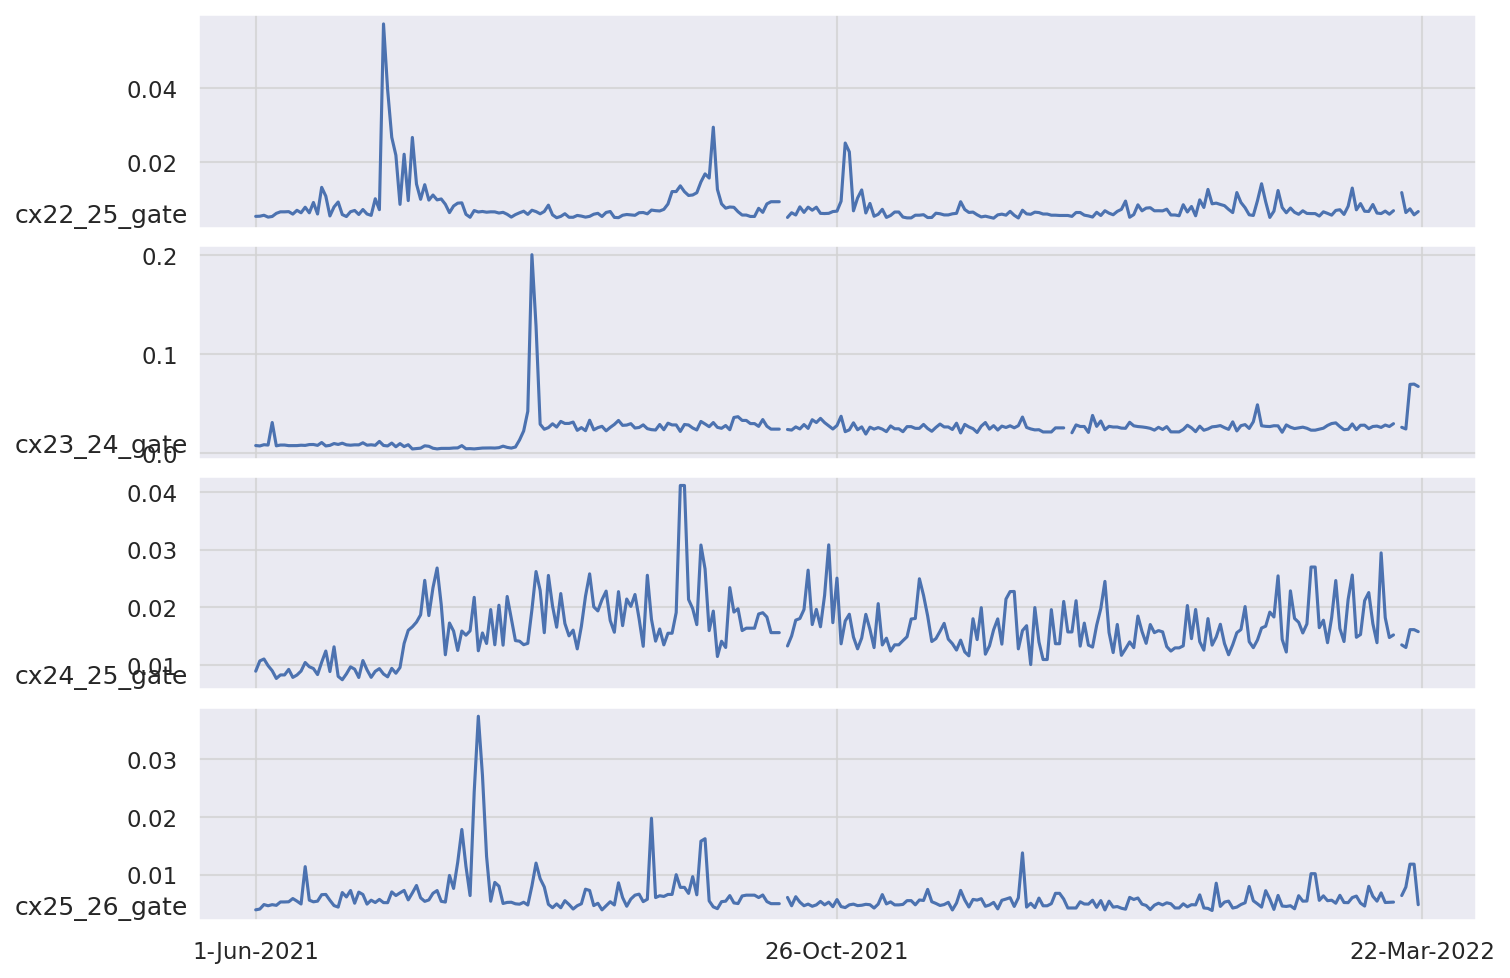
\includegraphics[width=0.64\columnwidth]{FG_raw_time_6.png}\label{fig:FG_raw_time_6}}
\hfil
\subfloat[Seven]{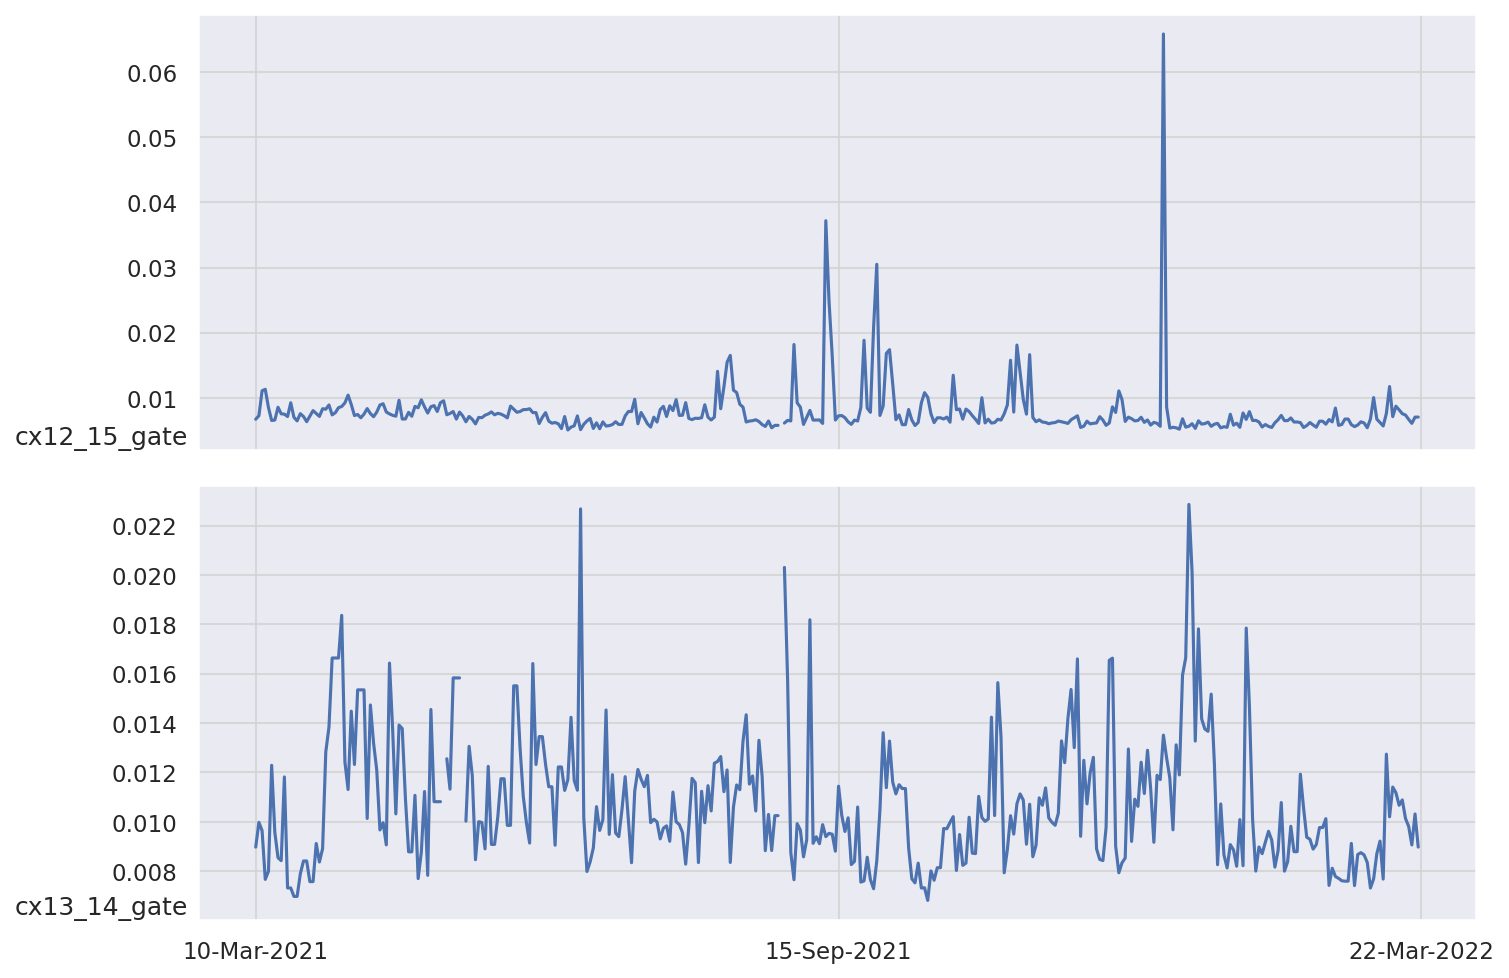
\includegraphics[width=0.64\columnwidth]{FG_raw_time_7.png}\label{fig:FG_raw_time_7}}

\caption{Characterizing the across-time variability of CNOT fidelity of \washington. The data in the 8 plots shown above cover all the permitted CNOT connections between nearest neighbour register pairs for the period 9 Dec, 2021 (when \washington was commissioned) to 8 Mar, 2022 (date of writing). The vertical axis represents the gate fidelity $\in [0, 1]$ expressed as percentage. The horizontal axis represents time.}
% of the \protect\subref{fig:yorktown} \yorktown and \protect\subref{fig:toronto} \toronto devices produced by IBM. Circles denote register elements and edges denote connectivity of 2-qubit operations.}
\label{fig:tbd1}
\end{figure*}
%%%%%%%%%%%%%%%%%%%%%%%%%%

\end{document}
